% !TEX program = pdflatex
%%%%%%%%%%%%%%%%%%%%%%%%%%%%%%%%%%%%%%%%%
% Structured General Purpose Assignment
% LaTeX Template
%
% This template has been downloaded from:
% http://www.latextemplates.com
%
% Original author:
% Ted Pavlic (http://www.tedpavlic.com)
%
% Note:
% The \lipsum[#] commands throughout this template generate dummy text
% to fill the template out. These commands should all be removed when
% writing assignment content.
%
%%%%%%%%%%%%%%%%%%%%%%%%%%%%%%%%%%%%%%%%%

%----------------------------------------------------------------------------------------
%	PACKAGES AND OTHER DOCUMENT CONFIGURATIONS
%----------------------------------------------------------------------------------------

\documentclass{article}

\usepackage{fancyhdr} % Required for custom headers
\usepackage{lastpage} % Required to determine the last page for the footer
\usepackage{extramarks} % Required for headers and footers
\usepackage{graphicx} % Required to insert images
\usepackage{subcaption}
\usepackage{lipsum} % Used for inserting dummy 'Lorem ipsum' text into the template

\usepackage[utf8]{inputenc}
\usepackage[ngerman,english]{babel}
\usepackage[T1]{fontenc}
\usepackage{breakurl}
\usepackage[hyphens]{url}
\usepackage{color}
\usepackage{float}
\usepackage{hyperref}
\usepackage{tabularx}
\usepackage{enumitem}
\usepackage{color, colortbl}
\usepackage[super]{nth}
\usepackage{wrapfig}
\usepackage{amsmath}

\usepackage[
	backend=biber,
	style=numeric-comp,
	natbib=true,
	url=false,
	doi=false,
	eprint=false,
	sorting=none,
	isbn=false]
	{biblatex}

\bibliography{references}

\addto\captionsenglish{
  \renewcommand{\contentsname}%
    {Table of Contents}%
}

% Margins
\topmargin=-0.45in
\evensidemargin=0in
\oddsidemargin=0in
\textwidth=6.5in
\textheight=9.0in
\headsep=0.25in

\linespread{1.1} % Line spacing
% Set up the header and footer
\pagestyle{fancy}
\lhead{} % Top left header
\chead{} % Top center header
\rhead{\firstxmark} % Top right header
\lfoot{\lastxmark} % Bottom left footer
\cfoot{} % Bottom center footer
\rfoot{Page\ \thepage\ of\ \pageref{LastPage}} % Bottom right footer
\renewcommand\headrulewidth{0.4pt} % Size of the header rule
\renewcommand\footrulewidth{0.4pt} % Size of the footer rule

\setlength\parindent{0pt} % Removes all indentation from paragraphs

\begin{document}
\setcounter{tocdepth}{2} % No subsubsections


%----------------------------------------------------------------------------------------
% TITLE PAGE
%----------------------------------------------------------------------------------------
\pagenumbering{gobble}
% \maketitle
\begin{titlepage}
  \centering
\includegraphics[width=5cm]{pictures/tumlogo}

  \vspace{2.5cm}
  \Huge{Trainingswissenschaften} \\
  \vspace{0.1in}\huge{Zusammenfassung}\\

  \Large
  \vspace{1.5cm}
  \begin{tabularx}{9cm}{r l}
    Author: & Thomas Pettinger\\
            & Nils Kunze\\
  \end{tabularx}

  \vfill
  \textbf{2016-07-20} \\
  \vspace{0.3in}\normalsize{Trainingswissenschaften}\\
  \vspace{0.03in}\normalsize{\textsc{Technische Universität München}}\\
  \vspace{1cm}

\end{titlepage}
%----------------------------------------------------------------------------------------


\newpage
\thispagestyle{empty}
\tableofcontents

\newpage
\pagenumbering{arabic}

%!TEX root = ../report.tex

\section{Einführung}

\subsection{Trainingswissenschaft}
\begin{itemize}

\item Leistungsfähigkeit: zeitlich überdauernde Eigenschaften eines Individuums
  \begin{itemize}
  \item Konditionelle Komponenten: Ausdauer, Kraft, Schnelligkeit, Beweglichkeit
  \item Informationelle Komponenten: Technik, Taktik
  \item Determinanten: Einzelfaktoren, die die Ausprägung einer (Teil-) Komponente bestimmen
  \end{itemize}
\item Realisation: Aktion zur Bewältigung einer Aufgabe im Sport
\item Training: Maßnahmen zur Steuerung der Leistungsfähigkeit
  \begin{itemize}
    
  \item Training ist die planmäßige und systematische Realisation von Maßnahmen (Trainingsinhalte und Trainingsmethoden) zur nachhaltigen Erreichung von Zielen (Trainingsziele)
im und durch Sport.
  \item Beanspruchung -> Beanspruchungsfolgen -> Adaption \item Unterscheidung zwischen konditionell und informationell
  \item Belastung: objektiv von Außen auf den Organismus wirkende Faktoren
  \item Belastungsnormative: Größen zur Beschreibung des Belastungsreizes (Intensität, Dauer, Umfang,\ldots)
  \item Beanspruchung: individuelle Reaktion des Organismus auf eine Belastung (z.B. gemessen über Herzfrequenz)
  \item Trainingsziele: Ausgewählte Komponenten der Leistungsfähigkeit
  \item Trainingsmethoden: Kombination von Belastungsnormativen zum Ansprechen der Determinanten
  \item Trainingsinhalte: Übungsgut zur Implementierung der Methodik
  \item Der Anwendungskontext von Training, beeinflusst die Ziele und damit die Inhalte und Methoden
  \end{itemize}
\item Leistung: Relativierung von Aktion und -ergebnis (bzw.\ im Wettkampf) an einer Norm
  \begin{itemize}
  \item Leistungsdiagnostik
    \begin{enumerate}
      \item Beschreibung der Realisation
      \item Bewertung der Realisation vor dem Hintergrund einer Norm
      \item Rückschluss auf die Leistungsfähigkeit
      \item Ableitung von Trainingszielen
    \end{enumerate}
  \end{itemize}
\end{itemize}

\newpage
%!TEX root = ../report.tex

\section{Ausdauer}
Definition: Ermüdungswiderstandsfähigkeit (konditionell und informationell) und Regenerationsfähigkeit

\subsection{Systematik}
\subsubsection{Belastungsdauer}
\begin{itemize}
  \item Kurzzeitausdauer (<35s)
  \item Mittelzeit-Ausdauer(35s - 8min)
  \item Langzeitausdauer (> 8min): LZA I: 8-30min, LZA II: 30min - 3h, LZA III: 3-9h, LZA IV: >9h
\end{itemize}

\subsubsection{Allgemeine vs spezielle Ausdauer}
\begin{itemize}
  \item Allgemeine Ausdauer: Grundlage für Regeneration, Training und Erholung und Voraussetzung für spezielles Training
  \item Spezielle Ausdauer: Wettkampfspezifische Ausdauer-Anforderungen (wichtiger für sportlichen Erfolg)
\end{itemize}

\paragraph{KsA: Koeffizient der speziellen Ausdauer}
= durchschnittliche 100m-Zeit obere Nachbarstrecke / durchschnittliche 100m-Zeit untere Nachbarstrecke

\subsection{Energiebereitstellung}
\paragraph{Mechanismen}
\begin{itemize}
  \item Systematik: Je nach Dauer und Intensität der Belastung wird Energie aus verschiedenen Substanzen gewonnen.
  \item Energiegewinnung aus Substrat:
    \begin{itemize}
      \item Energiefluss: Rate, mit der Energie zur Verfügung gestellt werden kann.
      \item Kapazität: Energievorrat
    \end{itemize}
  \item Problem: Maximale Energie nur kurzfristig verfügbar\\
    Dauerleistungsgrenze: ca 40\%
  \item Energiearten
    \begin{itemize}
      \item alaktazid (Cache (high transfer, low capacity))
      \item laktazid (Memory)
      \item aerob (Drive)
    \end{itemize}
\end{itemize}

\subsection{Determinaten der Ausdauer}
\begin{centering}
\begin{tabular}{m{0.2\textwidth} | m{0.3\textwidth} | m{0.3\textwidth}}
                          & Intensiv                                                         & Extensiv \\ \hline
     Energiespeicher      & Phosphat                                                         & Glykogen \\ \hline
     Enzymaktivityät      & Phosphatstoffwechsel Laktatabbau und -toleranz                   & Kohlenhydrat- und Fettstoffwechsel \\ \hline
     Muskulatur           & vortriebrelevante Muskulatur                                     & Haltearbeit verrichtete Muskulatur \\ \hline
     Sauerstoffversorgung & \multicolumn{2}{c}{Schlagvolumen, Kapillarisierung der Arbeitsmuskulatur, Blutmenge} \\ \hline
     Qualität der Technik & \multicolumn{2}{c}{Bewegungsökonomie} \\ \hline
     Psychische Eigensch. & \multicolumn{2}{c}{Durchhaltevermögen, ``Stehvermögen'', ``mentale Härte''} \\
\end{tabular}
\end{centering}

\subsection{Herz-Kreislauf}
\begin{itemize}
  \item Maximale Sauerstoffaufnahme - Normale Werte: 38-42 ml O2/(min x kg) (Frauen) und 44-50 ml O2/(min x kg) \\
    Spitzensportler: ca doppelte Werte
  \item Herzminutenvolumen (abhängig von Herzvolumen und Belastungsherzfrequenz)
    \begin{itemize}
      \item untrainiert: 20 l/min
      \item trainiert: 40 l/min
    \end{itemize}
  \item Blut (abhängig von Blutmenge und Sauerstoffbindungsfähigkeit)
\end{itemize}

\subsection{Methoden nach Trainingsbereichen}
\begin{centering}
\begin{tabular}{m{0.25\textwidth} | m{0.5\textwidth} | m{0.25\textwidth}}
   Trainingsbereich              & Primäres Ziel                                                                   & Methode \\ \hline
   Regeneration                  & Regenerationsbeschleunigung                                                     & Extensive Dauermethode \\ \hline
   Grundlagenausdauer 1          & Ausdauerfähigkeit niedriger Intensitätsbereich                                  & Intensive Dauermethode \\ \hline
   Grundlagenausdauer 2          & Ausdauerfähigkeit hoher Intensitätsbereich und physiol. Kapazitätserweiterungen & Intervallmethoden \\ \hline
   Wettkampfspezifische \newline Ausdauer & Ausdauerfähigkeit im Wettkampfbereich                                           & Wettkampfmethode \\
\end{tabular}
\end{centering}

\subsection{Belastungsmotive und Ausdauertraining}
\begin{itemize}
  \item Intensität: Stärke eines Einzelreizes
  \item Dauer: Wirkungsdauer eines Einzelreizes
  \item Umfang: Dauer \& Zahl der Reize/Trainingseinheit
  \item Dichte: Zeitliches Verhältnis zwischen Belastungs- und Erholungsphasen
  \item Häufigkeit: Zahl der Trainingseinheiten pro Trainingszeitraum
\end{itemize}

\subsection{Methoden im Überblick}
\begin{itemize}
  \item Dauermethode: Ununterbrochene Dauerbelastung mit geringer intensität und keinen Pausen
  \begin{figure}[H]
          \centering
          \begin{subfigure}[b]{0.4\textwidth}
            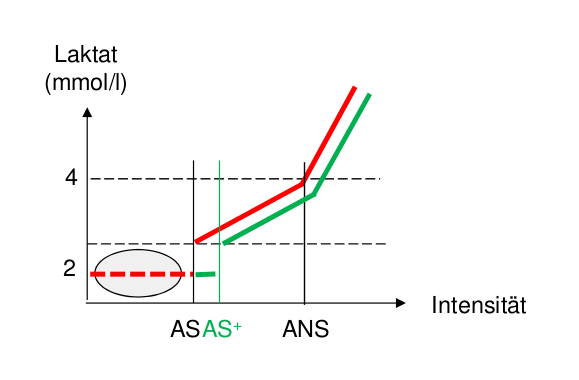
\includegraphics[width=\textwidth]{pictures/dauertraining_extensiv.png}
            \caption{Dauertraining extensiv}
          \end{subfigure}
          \begin{subfigure}[b]{0.4\textwidth}
            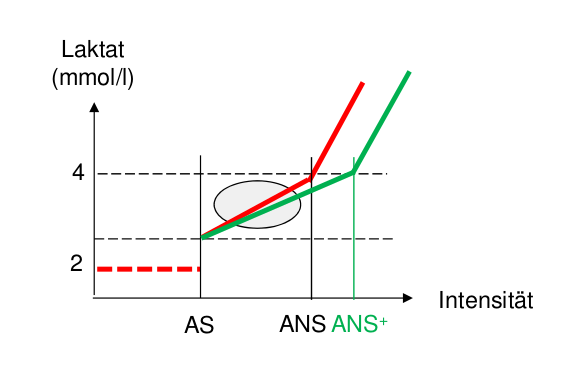
\includegraphics[width=\textwidth]{pictures/dauertraining_intensiv.png}
            \caption{Dauertraining intensiv}
          \end{subfigure}
        \end{figure}
    \begin{itemize}
      \item Extensiv: Intensität unterhalb der AS (?) \& Dauer von 20-60min oder mehr.\\
        Intension: Rechtsverschiebung der AS, Hoher Energieverbrauch, Regeneration, Gewöhnung an Belastungsmonotonie \\
      \item Intensiv: Intensität knapp unterhalb der ANS, Dauer \& Intensität hoch ($\leq$ ED)\\
        Intention: Rechtsverschiebung der ANS, Verbesserung des Glykose- und Laktatabbaus, Laktattoleranz (``MENTALE HÄRTE BITCH'')
    \end{itemize}
  \item Intervallmethoden: Intensität wechselnd über und unter dem ANS, durch Erholungspausen höhere Intensitäten als bei Dauermethoden mgl \\
    Intention: Verbesserung der Leistungsfähigkeit oberhalb der ANS, Phosphatstoffwechsel, hyperthrophie Herzmuskel (Belastungsphase), Erhöhung des Schlagvolumens
    \begin{figure}[H]
      \centering
      \begin{subfigure}[b]{.4\textwidth}
          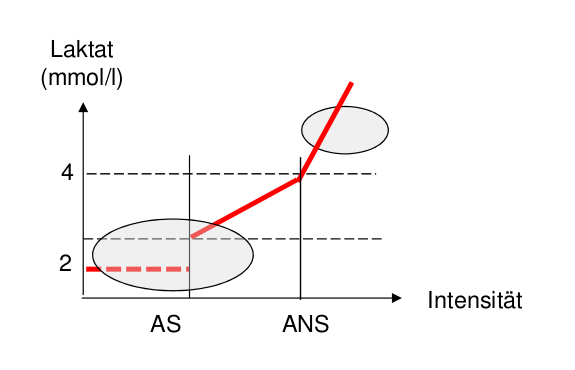
\includegraphics[width=\textwidth]{pictures/intervalltraining.png}
          \caption{Intervallmethoden}
      \end{subfigure}
      \begin{subfigure}[b]{.4\textwidth}
          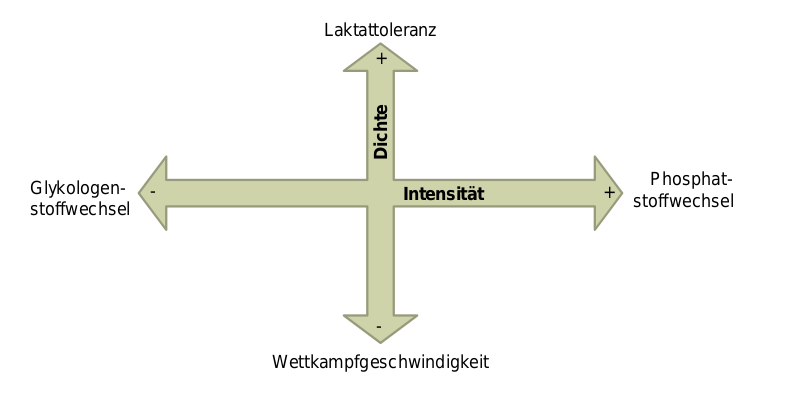
\includegraphics[width=\textwidth]{pictures/akzentuierung_der_trainingswirkung.png}
          \caption{Akzentuierung der Trainingswirkung}
      \end{subfigure}
    \end{figure}

\item Wiederholungsmethode: nahe maximale Intensität, ca. Wettkampfdauer, fast vollständige Pause\\
    Intention: Zusammenspiel aller Energiebereitstellungssysteme, alle physiologischen Prozesse
\item Wettkampfmehode: max. Intensität, mind. Wettkampfdauer, eine vollständige Pause \\
    Intention: Disziplinspezifische Belastungen, Validierung von Taktik, Trainieren der Superkompensation (d. Ausschöpfen von Reserven)\\
    Die Intensität wird beispielsweise durch Laufbandtests festgestellt, bei denen die Herzfrequenz bei erreichen der AS/ANS gemessen wird
\end{itemize}

\subsection{Trainingsinhalte}
Je nach Sportart und Leistungsziel werden andere Trainingsschwerpunkte gesetzt.
\begin{figure}[H]
    \centering
    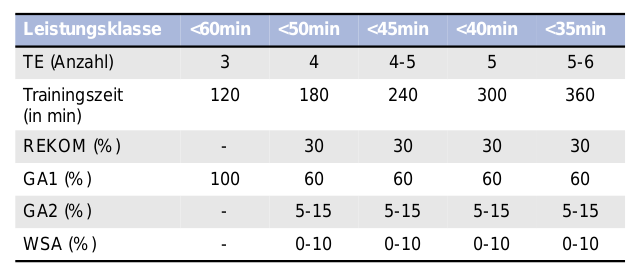
\includegraphics[width=.5\textwidth]{pictures/trainingsbeispiel_tempolauf.png}
    \caption{Trainingsbeispiel für einen Tempolauf über 10km}
\end{figure}

\subsection{Anwendung}
\begin{itemize}
    \item Leistungssport: (Ausdauer als Hauptanteil) REKOM, GA1, GA2, WSA
    \item Leistungssport (Ausdauer nicht Hauptanteil): REKOM (20min), GA1 (30-45min)
    \item Gesundheitssport: GA1 (min: 10-15min, opt: 30-45min)
\end{itemize}

Wirkungen auf die Gesundheit:
\begin{itemize}
    \item Geringere Belastung des Herzes im Alltag
    \item Höhere Resistenz für Infektion, Kälte \& Stress
    \item Positive Wirkung bei Depressionen
    \item Verbesserung der Gedächtnisleistung
    \item Erhöhter Kalorienumsatz
    \item Regulierung des Blutzucker- und Cholesterinspiegels
\end{itemize}
HIIT (High-intensity interval training) wird im Freizeitsport als unkritisch eingestuft.
Mit HIIT können kürzere Trainingszeiten für gleiche Effekte erzielt werden.

\subsection{Medizinische Empfehlung}
Sport wird ab einem Übergewicht von 20\% medizinisch empfohlen (Idealgewicht Körpergröße in cm - 100).
Das Training sollte langsam beginnen (optimal 70\% der maximalen Herzfrequenz), jedoch 10 Minuten 2-3 mal die Woche.
Bei Verbesserung der Leistung erst Häufigkeit und Belastungsumfang (jedoch nicht gleichzeitig), dann erst Intensität.

\subsection{Diagnostik}
\paragraph{Stufentest}
Der Stufentest ist ein Test für die aeroben Kapazität.
Ein Laufband wird benutzt bei dem alle 3 Minuten die Stufe erhöht wird (Anfang 60-100W, Stufe 20W).
Der Test wird abgebrochen wenn die Testperson subjektiv erschöpft ist oder eine festgelegte Geschwindigkeit erreicht wurde.
Mann misst dabei die AS und ANS mittels der Laktatkonzentration und die Geschwindikeit beim Abbruch.
\paragraph{Cooper-Test}
Der Cooper-Test testet die Ausdauerfähigkeiten einer Person.
Der Test besteht aus einem 12 Minuten Lauf bei dem die zurückgelegte Strecke gemessen wird.
Belastet werden dabei vor Allem die aerobe und anaerobe Energiebereitstellung.
\paragraph{Wingate Test}
Der Wingate Test zielt auf die anaeroben Kapazitäten ab.
Er besteht aus einem 30 Sekunden Sprint auf einem Radergometer mit konstant hohem Wiederstand.
Dabei werden die maximale Leistung, relative maximale Leistung, mittlere Leistung und Ermüdungsindex erfasst.
\paragraph{Yo-Yo-Test}
Der Test besteht aus 2x20m Lauf mit steigender Geschwindkeit, anschließend 2x5m Pause.
Der Lauf startet mit 10km/h mit einer Temposteigerung nach 8 Teilläufen um 0.5km/h.
Abgebrochen wird wenn zwei mal in Folge die Zeit nicht eingehalten.

\subsection{Zusammenfassung}
Ausdauertraining kann in jedem Alter ausgeführt werden und hat vielfältige positive Auswirkungen auf die Gesundheit.
Für optimales Training ist eine Kombination aus allgemeinem und spezifischen Methoden notwendig.
Die Grundlagen der Energiebereitstellung können eine Grundlage zum ausarbeiten eines Trainingsplans sein.

\newpage
%!TEX root = ../report.tex

\section{Kraft}

\begin{wrapfigure}{r}{0.5\textwidth}
    \begin{center}
        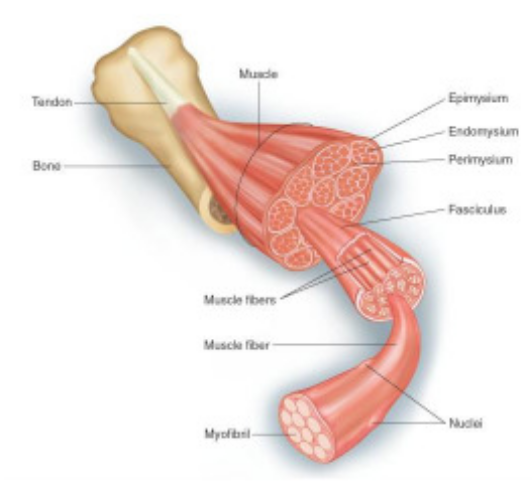
\includegraphics[width=0.48\textwidth]{pictures/muskeln}
    \end{center}
\end{wrapfigure}

Beispiele:
\begin{itemize}
    \item einmalig maximale Kraft (Gewichtheben)
    \item schnell und viel Kraft (Ringen, Hochsprung)
    \item Kraft aufrecht erhalten (Brücke)
\end{itemize}

Anatomische Grundlagen:
\begin{itemize}
    \item grundsätzlich drei Komponenten: Muskel, Sehne, Knochen
    \item Muskel bestehen aus:
    \begin{itemize}
        \item Muskelfaserbündel
        \item Muskelfaser
        \item Myofibrille
        \item Sarkomer
        \item Aktin-Myosin
    \end{itemize}
\end{itemize}

\begin{figure}[h]
\begin{tabular}{|c|c|c|c|}
 \hline
Kontraktionsform & Arbeitsweise & Ansatz / Ursprung & Beispiel Liegestütze \\ \hline \hline
konzentrisch & überwindend & Wird kleiner & Von Boden in Stütz \\ \hline
exzentrisch & nachgebend & Wird größer & Von Stütz auf Boden \\ \hline
isometrisch & haltend & Bleibt gleich & Halten des Stützes \\ \hline
\end{tabular}
\caption{Aktionsformen der Muskeln}
\end{figure}

\subsection{Struktur der Kraft}

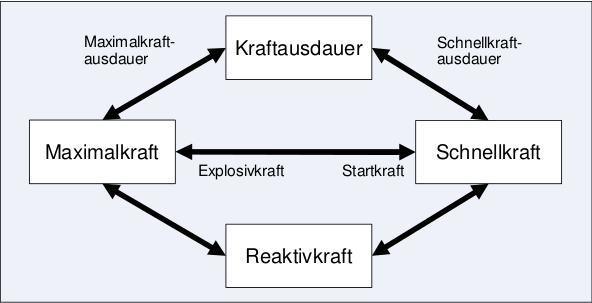
\includegraphics[width=0.9\textwidth]{pictures/kraftstruktur}

\subsection{Determinanten der Kraft}
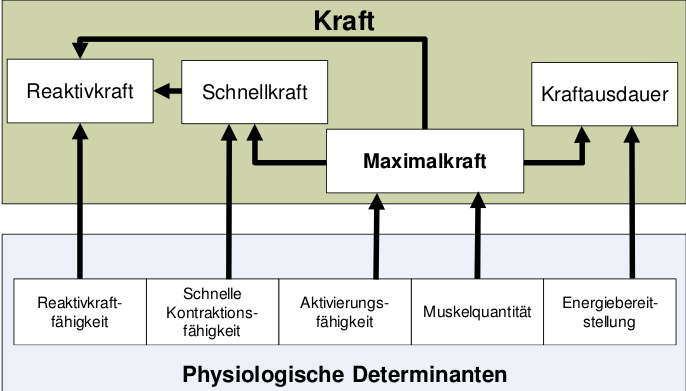
\includegraphics[width=0.9\textwidth]{pictures/kraft_determinanten}

\subsection{Maximalkraft}

[placeholder] % otherwise figure is not at correct position

\begin{wrapfigure}{r}{0.5\textwidth}
    \begin{center}
        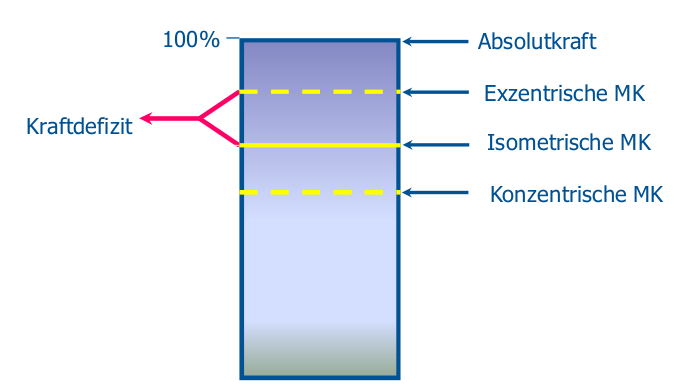
\includegraphics[width=0.48\textwidth]{pictures/maximalkraftvarianten}
    \end{center}
\end{wrapfigure}

[placeholder] % otherwise figure is not at correct position

\begin{itemize}
    \item Definition: Maximalkraft ist die höchstmögliche Kraft, die vom Nerv-Muskel-System willentlich gegen einen Widerstand erzeugt werden kann
    \item 1er-Maximum (1RM = 1 Repetition Maximum) = konzentrische Maximalkraft über volle Bewegungsamplitude
    \item Relativkraft = 1RM / Körpergewicht
    \item bestehend aus:
    \begin{itemize}
        \item Muskelquerschnitt \& Faserzusammensetzung
        \item Willkürliche Aktivierungsfähigkeit
    \end{itemize}
    \item Absolutkraft: Nur durch maximale elektrische Stimulation erreichbare Kraft. Willentlich nicht abrufbar.
    \item Kraftdefizit: $\frac{\text{Exzentrische MK} - \text{Isometrische MK}}{\text{Exzentrische MK}} \cdot 100 \%$
    \item in Praxis: Differenz zwischen isometrischer und exzentrischer MK
    \item Training:
    \begin{itemize}
        \item großes Kraftdefizit: willkürliche Aktivierungsfähigkeit verbessern
        \item kleines Kraftdefizit: Muskelquantität
    \end{itemize}
\end{itemize}

\subsection{Schnellkraft}

[placeholder] % otherwise figure is not at correct position
\begin{wrapfigure}{r}{0.5\textwidth}
  \begin{center}
    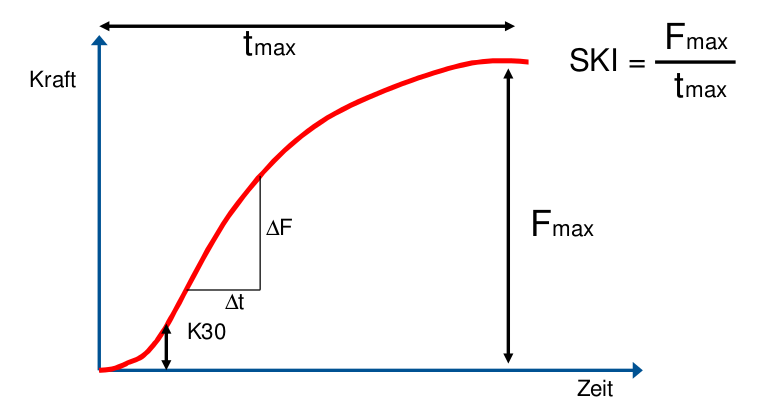
\includegraphics[width=0.48\textwidth]{pictures/kraftanstiegskurve}
  \end{center}
\end{wrapfigure}

\begin{itemize}
    \item Definition: Schnellkraft ist die Fähigkeit, einen möglichst großen Kraftstoß innerhalb einer zur Verfügung stehenden (kurzen) Zeit zu realisieren
    \item Teilaspekte:
    \begin{itemize}
        \item Startkraft (Fähigkeit sehr schnell Kraft zu entfalten, bsp: Boxen?)
        \item Explosivkraft (Fähigkeit großen/schnellen Kraftanstieg zu realisieren, bsp: Würfe, Stöße, Schüsse?)
        \item Dynamisches Kraftmaximum (Fähigkeit MK schnell zu realisieren, bsp: Ringen?)
    \end{itemize}
    \item Struktur der Schnellkraft: Maximalkraft + Schnelle Kontraktionsfähigkeit
    \item Schnelle Kontraktionsfähigkeit hängt ab von Muskelfaserzusammensetzung, Intermuskulärer und Intramuskulärer Koordination
\end{itemize}

\paragraph{Muskelfaserzusammensetzung}
\begin{itemize}
    \item Zusammensetzung genetisch determiniert
    \item Umwandlung praktisch nur Fast Twitch to Slow Twitch durch Ausdauertraining und Querschnittstraining
\end{itemize}
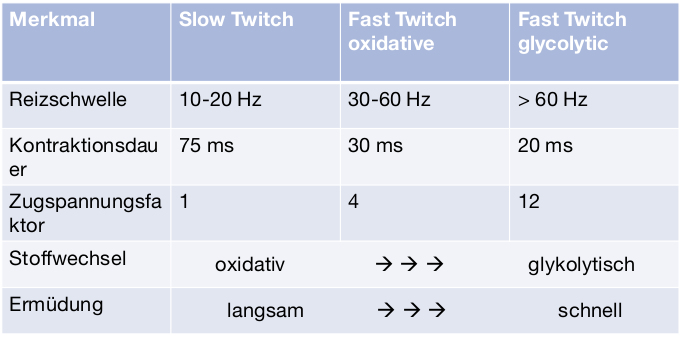
\includegraphics[width=0.9\textwidth]{pictures/muskelfaserzusammensetzung}

\paragraph{Intermuskuläre Koordination}
\begin{itemize}
    \item Zusammenspiel mehrerer Muskeln (Muskelabschnitte)
    \item fertigkeitsspezifisch
    \item kann als Synonym für ``Gute Technik'' betrachtet werden
    \item Grund warum Krafttraining nicht nur auf Stärkung der einzelnen Muskeln ausgelegt sein darf
    \item Beispiele: Fuß-, Knie- und Hüftstrecker bei Strecksprung
\end{itemize}

\paragraph{Intramuskuläre Koordination}
\begin{enumerate}
    \item Sequenzierung: Optimale Reihenfolge der Innervation der Muskelfasern
    \item Frequenzierung: Fähigkeit, den Muskel hochfrequent und nachhaltig zu innervieren
    \begin{itemize}
        \item Je nach Stärke der Erregung über die spinalen Synapsen, feuert ein Motoneuron mit unterschiedlicher Frequenz
        \item  Ab 55 Hz wird Maximale Kraftabgabe möglich
        \item  Bis zu 155 Hz sind möglich und erlauben schnellen Kraftanstieg
    \end{itemize}
    \item Rekrutierung: Fähigkeit, möglichst viele motorische Einheiten zur Kontraktion heranziehen zu können

\newpage
%!TEX root = ../report.tex

\section{Schnelligkeit}
Schnelligkeit ist die Fähigkeit in ermüdungsfreiem Zustand mit möglichst kurzen zeitlichem Abstand auf einen Reiz zu reagieren oder zu agieren.
\begin{figure}[H]
  \centering
  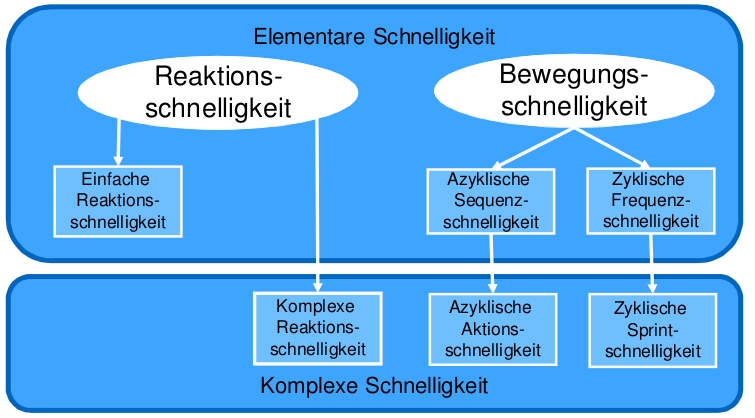
\includegraphics[width=.5\textwidth]{pictures/schnelligkeit_overview.png}
  \caption{Überblick Schnelligkeit}
\end{figure}
\begin{figure}[H]
  \centering
  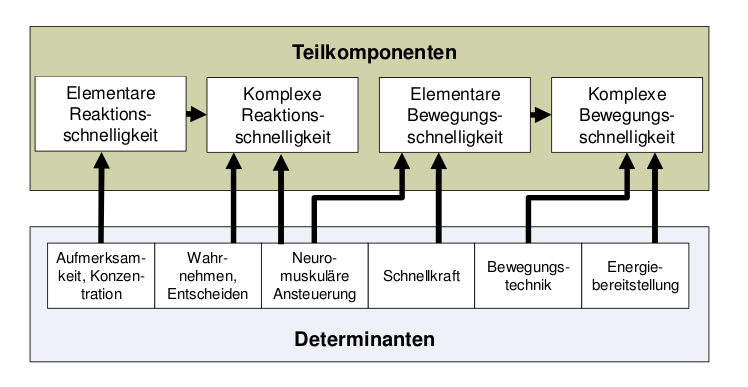
\includegraphics[width=.5\linewidth]{pictures/schnelligkeit_determinanten.png}
  \caption{Determinanten der Schnelligkeit}
\end{figure}

\subsection{Begriffe, Systematik und Determinaten}
\subsubsection{Reaktionsschnelligkeit}
\begin{description}
  \item[Reaktionsfähigkeit] ist die psychophysische Fähigkeit auf Reize schnell zu reagieren.
  \item[Elementare Reaktionsschnelligkeit] Kleinmotorische Bewegungsantworten auf einfache Reize
  \item[Komplexe Reaktionsschnelligkeit] Großmotorische Bewegungsantworten \& komplexe (Wahl-) Reaktionen.
\end{description}

\textbf{Modell der Reaktionsgeschwindigkeit}\\
\begin{figure}[H]
  \centering
  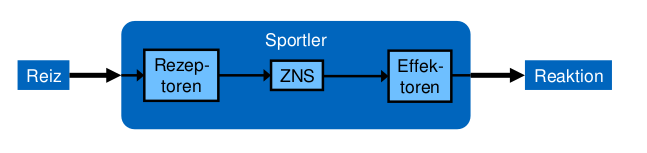
\includegraphics[width=.5\textwidth]{pictures/reaktionsgeschwindigkeit_modell.png}
  \caption{Modell der Reaktionsgeschwindigkeit}
\end{figure}
\begin{description}
    \item[Übertragung bis Rezeptor] hängt vorwiegend von den Eigenschaften des Rezeptors ab (1-20ms).
    \item[Restliche ÜBertragung] wird von den Eigenschaften des Nervensystems beeinflusst (Rezeptor $\rightarrow$ ZNS: 1-100ms, ZNS $\rightarrow$ Effektor: 10-20ms).
    \item[Verarbeitung im ZNS] wird beeinflusst von psychischen Eigenschaften wie Aufmerksamkeit und Wahrnehmung und kann von 70 bis 300ms dauern.
    \item[Verarbeitung in den Effektoren] Abhängig von neuromuskulären Eigenschaften wie Fastetypzusammensetzung oder inter-/intramuskuläre Koordination
\end{description}
Die gesammte Übertragungszeit beträgt in etwa 112 - 510ms.

\subsubsection{Bewegungsschnelligkeit}
Bewegungsschnelligkeit ist die Fähigkeit, Bewegungen in höchster Geschwindigkeit oder kürzester Zeit auszuführen.
\begin{figure}[H]
    \centering
    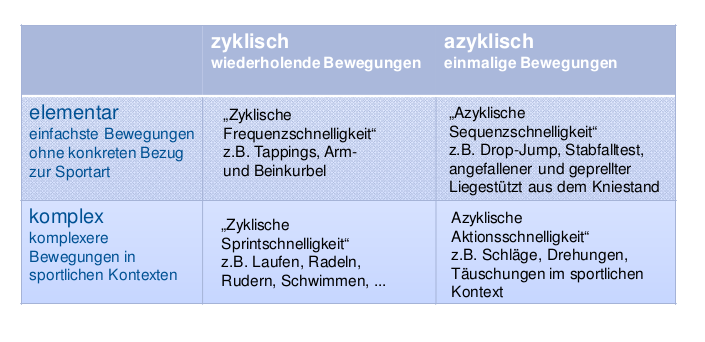
\includegraphics[width=.7\textwidth]{pictures/bewegungsgeschwindigkeit_struktur.png}
    \caption{Struktur der Bewegungsschnelligkeit}
\end{figure}

Die Bewegungsschnelligkeit hängt von drei Bereichen ab:
\begin{description}
    \item[Neuromuskuläres System] Neuronale Steuer- \& Regelprozesse, Reaktionsgeschwindigkeit, inter/intra-muskuläre Koordination,\ldots
    \item[Psychisches System] Konzentration, Wahrnehmung, Motivation, \ldots
    \item[Tendomuskuläres System] Querschnittsfläche FT-Fasern, Stiffness, Viskosität, \ldots
\end{description}

\subsection{Trainingsmethoden}
Schnelligkeit ist schlechter zu trainieren als Ausdauer oder Kraft.\\
Zu trainierende Determinanten sind:
\begin{figure}[H]
    \centering
    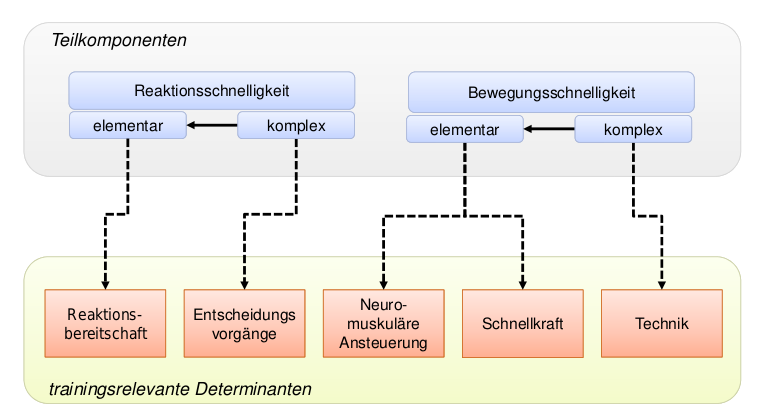
\includegraphics[width=.7\textwidth]{pictures/schnelligkeit_trainierbare_determinanten.png}
    \caption{Trainierbare Determinanten}
\end{figure}

\paragraph{Belastungsnormative}
\begin{description}
    \item[Intensität] Bewegung auf maximaler Geschwindigkeit
    \item[Dauer] 8-10s, Abbruch bei Erschöpfung
    \item[Pause] bis vollständig regeneriert, Schnelligkeitstraining vor anderen
    \item[Durchführung] Mit maximaler Konzentration \& Willen, mit Aufwärmen
\end{description}

\subsubsection{Reaktionsbereitschaft}
Training beinhaltet einfache Reaktionen (Pfiff, (Nacken- :P) Klatschen) auf akustische, visuelle oder taktile Reize.

\subsubsection{Entscheidungsvorgänge}
Eine Wahlreaktion wird vor einer motorischen Reaktion eingefordert.
Auch die richtige Wahrnehmung ist wichtig, Signal wird erschwert zu verstehen (leiser Pfiff = noop, lauter Pfiff = go)

\subsubsection{Neuromuskuläre Ansteuerung}
Grundbewegungen schnell realisieren. Es wird unterschieden zwischen zyklischen (wiederholenden) und azyklischen (einmaligen) Bewegungen.
\paragraph{Geschwindigkeitsbarriere} Häufige Realisation der Maximalgeschwindigkeit führt zu einer Verfestigung der neuromuskulären Ansteuerung (Reizleitungswege, Innervationsmuster).
Gegenmaßnahmen sind nur wenig Wettkampfsimulationen mit Maximalgeschwindigkeit (1/Woche), Variation der Bewegung und Entwicklung der elementaren Fähigkeiten
\paragraph{Erleichterte Bedingungen} Erleichtern der Übungen durch verringern des Wiederstands oder Körpergewichts um Geschwindigkeit zu erhöhen.
Beispiele sind Treppenläufe bergab (zyklisch) oder leichtere Wurfgeräte (azyklisch).
\paragraph{Räumliche Zwänge} Erzwingen einer höheren Frequenz durch Einengungen (z.B. Fesseln).
\paragraph{Mentales Training} Der Carpenter-Effekt (Denken an eine Bewegung bewirkt diese in einem abgeschwächtem Maß) wird dazu genutzt mit Metaphern in der Übungsbeschreibung eine Aktion hervorzurufen (``Springe wie ein Frosch'').
\paragraph{Elektromyostimulation} Elektrische Stimulation auf das Innervationsmuster. Die nicht belegte Hypothese ist dass dadurch eine bessere Rekrutierung motorischer Einheiten erfolgt und das bestehende Innervationsmuster ``überschrieben'' wird.

\subsubsection{Technik}
Technikübungen sind disziplinspezifisch, schnell ausgeführte Bewegungen die meist überbetont werden.
Kombinationen aus einzelnen Aktionen und Übungen sind möglich.

\subsubsection{Schnellkraft}
Eine Erschwerung der Bedingungen (z.B. Laufen mit Zugschlitten) führt zu einem Training für Kraft und Schnelligkeit.
Dadurch ist allerdings die maximale Geschwindigkeit nicht mehr zu erreichen.

\newpage
%!TEX root = ../report.tex

\section{Beweglichkeit}

Definition Beweglichkeit: Beweglichkeit ist die motorische Fähigkeit, Bewegungen willkürlich mit der erforderlichen Schwingungsweite ausführen zu können.

Verwandte Begriffe: \textbf{Gelenkigkeit} = Schwingungsweite von Gelenken, \textbf{Dehnfähigkeit} = Dehnbarkeit von Muskeln und Sehnen

Optimalitätseigenschaft: Stabilität versus Mobilität, Hypo- versus Hypermobilität

\subsection{Systematik und Determinanten}

\subsubsection*{Dimensionen }

\begin{minipage}{0.7\textwidth}
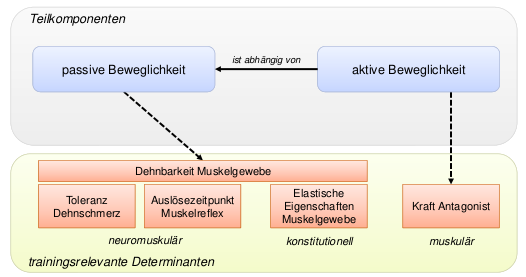
\includegraphics[width=\textwidth]{pictures/beweg_determinanten4}
\end{minipage}
\begin{minipage}{0.3\textwidth}
\begin{itemize}
    \item Passive Beweglichkeit: Beweglichkeit die unter Einwirken einer externen Kraft erreicht wird (z.B. Spagat, Schwerkraft)
    \item Aktive Beweglichkeit: Beweglichkeit, die durch aktive Muskelarbeit erreicht wird (z.B. Armschwung, Schuss, Spagatsprung)
\end{itemize}
\end{minipage}

Methoden im Beweglichkeitstraining:
\begin{itemize}
    \item aktiv: Antagonisten bewirken Dehnung
    \item passiv: Partner, Schwerkraft, andere Muskeln bewirken Dehnung
    \item statisch: langsames Einnehmen der Dehnposition, ohne Auslösung des Muskelreflexes (intensiv)
    \item dynamisch: schnelles, federndes Einnehmen der Dehnposition, mit (unter Inkaufnahme der) Auslösung des Muskelreflexes
\end{itemize}

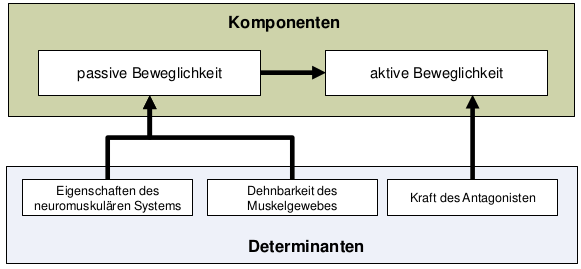
\includegraphics[width=0.9\textwidth]{pictures/beweg_determinanten2}

\subsubsection*{Muskelreflex}

Schnelle Bewegungen lösen den Muskelreflex aus, aber das Auslösen des Muskelreflexes ist kontraproduktiv zur Absicht der Dehnung. Wenn die Dehnung intensiv sein soll, sollte Muskelreflex nicht (nur minimal) ausgelöst werden, d.h. keine schnellen Bewegungen.

Der Muskeltonus ist Ausdruck des systemischen Erregungszustandes. Zu hoch impliziert sanfte Dehnung und Entspannungsübungen, zu niedrig dagegen intensive Dehnung.

Allgemein:
Ein Gelenk besteht aus Muskeln und Sehnen, Knochen, Knorpel und der Gelenkkapsel mit Bändern.
Es gibt verschiedene Rezeptoren:
\begin{itemize}
    \item Ruffini-Körperchen sind Mechanorezeptoren in Kapsel und Haut und reagieren auf Druck und Dehnung. Dabei registrieren sie das Ausmaß und die Geschwindigkeit von Gelenkbewegungen.
    \item Vater-Pacini-Körperchen sind Mechanorezeptoren im Gelenkbindegewebe und registrieren Beschleunigungen.
    \item Golgi-Sehnenorgan sitzt im Übergang zwischen Muskeln und Sehnen und registriert dort die Muskelspannung. Unter Umständen gibt es eine Reflexantwort.
    \item Muskelspindeln sind quergestreifte Muskelfasern, die ebenfalls als Mechanorezeptoren dienen. Sie lösen den Eigenreflex aus und messen das Ausmaß und die Geschwindigkeit einer Muskelbewegung.
\end{itemize}

\subsubsection*{Determinanten}

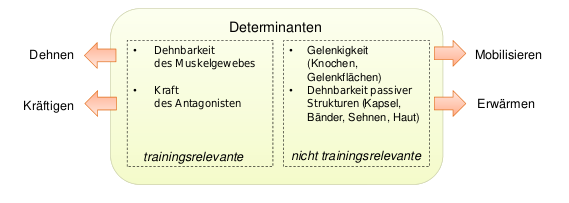
\includegraphics[width=\textwidth]{pictures/beweg_determinanten3}

\begin{minipage}{0.4\textwidth}
Entscheidend sind folgende anatomische Eigenschaften:
\begin{itemize}
    \item Freiheitsgrade und Funktionstüchtigkeit der Gelenke
    \item Bandhafte- und kapsuläre Hemmung
    \item Titinfilamente (hauptsächlich verantwortlich für Widerstand)
    \item Tendo-muskuläre Reflexschaltungen (Hemmungen)
\end{itemize}
\end{minipage}
\begin{minipage}{0.6\textwidth}
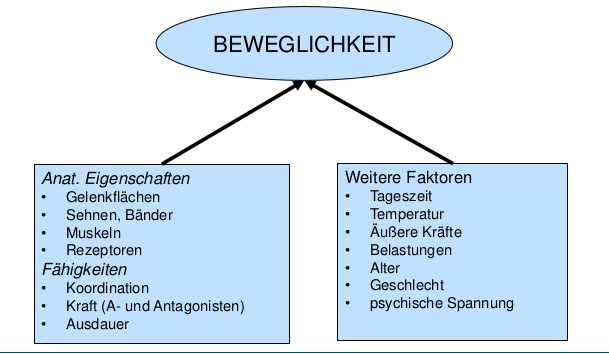
\includegraphics[width=\textwidth]{pictures/beweg_determinanten}
\end{minipage}
Weitere Einflussfaktoren:
\begin{itemize}
    \item Alter: Abnahme der Elastizität (H 2 O-Verlust; Weniger Zellen)
    \item Geschlecht: Einfluss des Östrogens
    \item Ausdauer: Kein Beweglichkeitstraining im Ermüdungszustand
\end{itemize}

\subsection{Bedeutung}

Beweglichkeit kann Bestandteil von Wettkampfleistungen sein (Bsp: bessere Bepunktung von Spagat in der Gymnastik) oder Voraussetzung für Wettkampfleistungen, konditionelle Fähigkeiten oder Teilleistungen sein (Bsp: bessere performance von beweglicheren Fußballspielern).

Als Beweglichkeitsreserve bezeichnet man die Differenz zwischen erforderlichem und maximalem Bewegungsausschlag. Eine große Reserve ist erstrebsam, weil dann nicht bis an die Dehnbarkeitsgrenze belastet werden muss (Ökonomisierung) und die Bewegung unter geringerem Widerstand ablaufen kann. Auch im Fitness- und Gesundheitstraining ist Dehnen zur Vermeidung von Dysbalancen und Verkürzungen relevant.

\subsubsection*{Aufwärmen vs Dehntraining}

Seit Mitte der 90er Jahren ist bekannt, dass intensives statisches Dehnen (Stretching) in der Aufwärmphase genau das Gegenteil von dem, was man sich erhofft, bewirkt.
Statt leistungssteigernd und verletzungsmindern zu wirken, führt es zu geringerer Leistung und einem größerem Verletzungsrisiko. Ausmaß: 4-8\% weniger vertikale Sprungleistung und 5-10\% Reaktivkraftleistungen

Gründe:
\begin{itemize}
    \item Geringere Kraftproduktion Muskel-Sehnen-Komplex (Verlängerung, Belastung der fibrillären Strukturen)
    \item Periphere neuromuskuläre Veränderungen, z.B. Reduktion der
    \item Erregbarkeit der Motoneurone
    \item Zentrale psychophysiologische Desaktivierungsprozesse, Senkung der zentralen Aktivierung
\end{itemize}

Verletzungsprophylaxe: Kräfte bei passiver Dehnung können sehr groß und unphysiologisch werden, zusätzliche steht ein epidemiologischer Nachweis der Verletzungsprophylaxe-Wirkung von intensivem Dehnen noch aus. Muskelkater kann durch (zu) intensives Dehnen verschlimmert bzw. sogar herbeigeführt werden...

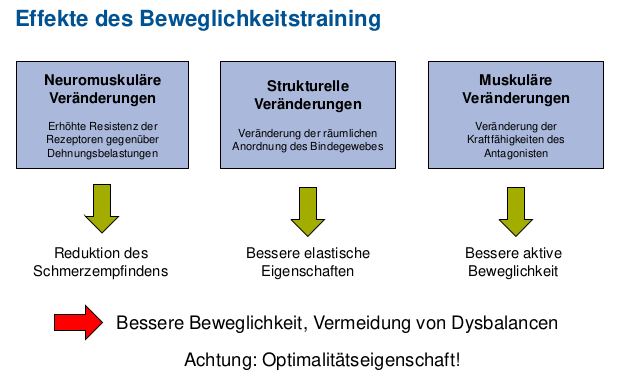
\includegraphics[width=0.9\textwidth]{pictures/beweg_effekte}

\subsection{Diagnostik}

Motorische Beweglichkeits-Tests z.b. mit ablesen auf einer Zentimeterskala und abgleich gegen Normtabelle. Problem von Normwerten: Liefern nur erste Hinweise

Ein anderes klassisches Verfahren zur einfachen Bestimmung von Beweglichkeitseinschränkungen in der Muskulatur  ist der Janda-Test.
Beispiel für den Hüftlendenmuskel: Rückenlage, Oberschenkel beugen und Richtung Brust heranziehen, dabei muss die Lendenwirbelsäule komplett aufliegen.
Anzeichen für Beweglichkeitseinschränkung: der Oberschenkel der Gegenseite geht nach oben.

\subsection{Trainingsmethoden}

\paragraph*{Belastungsnormative}
Problem: Wie wählt man die Intensität? \% des maximalen Bewegungsumfangs? Subjektives Rating über Schmerzskala?
Dauer, Umfang, Dichte, Häufigkeit weniger wichtig, entscheidend ist die Ausführungsart.

Ausführungsarten:
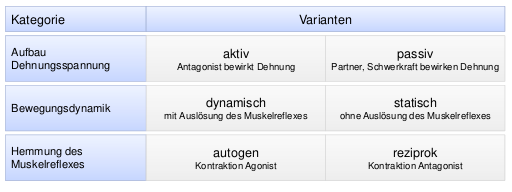
\includegraphics[width=0.9\textwidth]{pictures/beweg_ausfuehrungsarten}

Static Stretching (SS):
\begin{itemize}
    \item Langsame Heranführung an Bewegungsgrenze bewirkt Hemmung des Dehnungsreflexes der Muskeln und Sehnenspindeln
    \item Einnehmen der Dehnposition, so dass deutliche
    Spannung spürbar ist ( = Andehnen).
    \item Wenn das Spannungsgefühl nachlässt, Verstärkung der Dehnung und erneutes Halten ( = Nachdehnen).
    \item Dauer: zwischen 5s und > 60s (je nach Trainingsziel)
\end{itemize}

Contract Relax (CR):
\begin{itemize}
    \item vorgeschaltete Kontraktion des Agonisten führt zur Hemmung des Dehnungsreflexes des Agonist (autogene Hemmung)
    \item Isometrische Kontraktion (submaximal bis maximal) des Agonisten (5s) (C=Contract)
    \item Entspannen des Agonisten (2s) (R=Relax)
    \item Dehnen des Agonisten (aktiv oder passiv)
    \item auch Contract-Hold-Release-Stretch (CHRS) genannt
\end{itemize}

Antagonist Contract (AC):
\begin{itemize}
    \item vorgeschaltete Kontraktion des Antagonisten führt zur Hemmung des Dehnreflexes des Agonisten (reziproke Hemmung)
    \item Anspannen des Antagonisten (5s) (AC)
    \item Dehnen des Agonisten (aktiv oder passiv)
    \item Anspannen und Dehnen, gleichzeitig oder sequenziell
\end{itemize}

Contract Relax – Antagonist Contract (CR-AC):
\begin{itemize}
    \item Ausnutzung beider Effekte
    \item Kontraktion des Agonisten (C)
    \item Entspannung (R)
    \item Dehnen des Agonisten mittels Kontrakation des Antagonisten (AC)
    \item aktiv oder passiv
    \item auch PNF-Dehnen genannt (Propriozeptive neuromuskuläre Fazilitation)
\end{itemize}

Dynamic Stretching (DS):
\begin{itemize}
    \item Nutzung von Schwungkräften
    \item Wiederholtes federn an die Bewegungsgrenze ( = Balistics) oder
    \item langsames „Schieben“ an die Bewegungsgrenze, kurz halten ( = Ballistic \& Hold)
    \item Vorteile: gleichzeitige Kräftigung des Antagonisten und Verbessern der aktiven Beweglichkeit
    \item Nachteile: Dehnreflex, weniger intensive Dehnung möglich
\end{itemize}

\subsection{Trainingsinhalte}

Generelle Hinweise:
\begin{itemize}
    \item Mobilisierung und Aufwärmen vor dem Dehnen
    \item Dehnen möglichst selektiv (eingelenkig)
    \item Beim Dehnen über zwei Gelenke: ein Gelenk fixieren
    \item Keine Dehnung von Muskeln die Haltearbeit leisten müssen
    \item Übungen so wählen, dass Ausweichbewegungen vermieden werde Reihenfolge einhalten
\end{itemize}

Kinder- und Jugendtraining: Eher aktive un dynamische Dehnübungen, Verzicht auf passive und statische Übungen. Außerdem Altergemäß durch Wettbewerbe oder Staffelspiele

\subsection{Anwendung}

Beweglichkeitsmaximierung:
\begin{itemize}
    \item Anwendung: (Hoch-)Leistungssport mit Beweglichkeit als leistungsbegrenzendem Faktor
    \item Methode: CR-AC>AC>CR>SS>DS (nicht nachgewiesen)
    \item Intensität: Maximal (bis an Schmerzgrenze), Einhalten von Belastungsgrenzen!
    \item Dauer: Bindegewebsanpassungen ab ca. 30s (Creeping)
    \item Umfang \& Häufigkeit: eigener Trainingsinhalt , 4-10 Serien, 1-2 Mal täglich, stabile Anpassungen nach ca. 6 Wochen
\end{itemize}

Beweglichkeitserhalt:
\begin{itemize}
    \item Anwendung: sonstiger Leistungssport, Gesundheits- und Freizeitbereich, Leistungsabfall ab 8. Lebensjahr!
    \item Methode: DS (evtl. SS), Dynamisches Dehnen kräftigt zusätzlich!
    \item Intensität: hoch, jedoch nicht bis an die Schmerzgrenze
    \item Dauer: 10-15s in Endposition oder 10 Mal wippen
    \item Umfang \& Häufigkeit: 2-3 Sätze pro Gelenk, 2-3 Mal pro Woche
\end{itemize}

Aufwärmen:
\begin{itemize}
    \item Anwendung: Sportarten in denen Beweglichkeit Vorteile bringt
    \item Pro-Argumente: kurzfristige Gewinne durch Dehnen erzielbar (ca. 8\%)
    \item Effekt der Verletzungsprophylaxe unklar
    \item Contra-Argumente (SS): Fast gleiche Gewinne an Bewegungsreichweite wie beim dynamischen Dehnen, Gefahr von Überlastungen, Durchblutung vermindert und Schnellkraftleistungen sinken kurzzeitig
    \item Methode: DS bevorzugen
    \item Intensität: mittel bis hoch
    \item Dauer: <5s bei maximal- und schnellkraftentwickelnder Muskulatur
    \item 10-15s bei beweglichkeits-relevanter Muskulatur
    \item keine Laktatanhäufung bei aktiven Methoden
    \item Umfang \& Häufigkeit: 1-3 Serien, 15-20 Minuten vor dem Wettkampf
\end{itemize}

Krampfbeseitigung:
\begin{itemize}
    \item Anwendung: Während der Sports, Bei Krämpfen verursacht durch Ermüdung oder mangelnde Versorgung (Blut, Mineralien)
    \item Methode: Vorsichtiges statisches Dehnen des Agonisten (SS) bevorzugen, Kontraktion des Antagonisten
    \item Intensität: gering
\end{itemize}

Cool-Down:
\begin{itemize}
    \item Anwendung: Verbesserung „Körpergefühl“,Verbesserung der Entspannungsfähigkeit,Abbau von Muskelverspannungen,Beschleunigung der Regeneration,Wirkung umstritten!
    \item Methode: SS bevorzugen, alternativ CR
    \item Intensität: eher niedrig bis mittel, sonst "Spülfunktion“ beeinträchtigt
    \item Umfang: 3 Serien nach dem Auslaufen, 5-10s inEndposition halten
\end{itemize}

\subsection{Exkurs: Aufwärmen \& Cool Down}

Aufwärmen:
\begin{itemize}
    \item Varianten:  allgemein vs. speziell, aktiv vs. passiv, physisch vs. mental
    \item Primäreffekte: Anregung Herz-Kreislaufsystem(Kerntemperatur, Atmung, Puls, Blutdruck), Durchblutung Muskultur, Flüssigkeitsregulation Knorpelgewebe
    \item Gewünschte Wirkung: Physische Leistungssteigerung(Sauerstoffversorgung, Erregbarkeit,Muskelviskosität, ...), Verletzungsprophylaxe, Psychische Aspekte
    \item Typisches Aufwärmprogramm (Volleyball): Kreislaufaktivierung, Mobilisation, (Dehnen), Stabilisation, Kurze hochintensive Belastung, Spezielles Aufwärmen mit Ball. Dabei keine Ermüdung induzieren!
\end{itemize}

Mobilisation:
\begin{itemize}
    \item Aufwärmen von Bindegewebe (Bänder, Gelenkkapsel)
    \item Verbesserung der Gleiteigenschaften des Gelenkes
    \item Amplitude nicht ausschöpfen, Funktionsweise des Gelenkes beachten
    \item ca. 5 Minuten vor dem Training
\end{itemize}

Stabilisation:
\begin{itemize}
    \item Kontraktion im Rumpf vor Bewegung (Feed-Forward)
    \item Schutzfunktion für die Wirbelsäule
    \item Biomechanische Vorrausetzung für Wurf-, Schlag-, Schussbewegungen
    \item Belastungsnormative: niedrigen Intensitäten (25\%), recht lange (30s), statisch und dynamisch, keine Periodisierung, trainingsbegleitend
\end{itemize}

Cool Down:
\begin{itemize}
    \item Ansatz: Langsame Normalisierung physischer und psychischer Parameter, Entlastung passiver Bewegungsapparat
    \item Gewünschte Wirkung: Beschleunigte Regeneration durch Beseitigung von toxischen Nebenprodukten, Lösung von Muskelverspannungen, Psychoregulation
\end{itemize}

Muskelkater:
\begin{itemize}
    \item Wahrscheinliche Ursache: Zerstörung von Sarkomer-Strukturen
    \item Dehnen eher kontraproduktiv
    \item Massage eher kontraproduktiv
    \item Wärmebehandlung zur Krampflockerung und Ödemausschwemmung
    \item Ruhigstellung und Schonung, keine hohen Kraftbelastungen
\end{itemize}

\subsection{Zusammenfassung}

\begin{itemize}
    \item „Leiche im Keller“ der TRW
    \item Pro-Argumente Dehnen: Erhaltung und Verbesserung Beweglichkeit (Beweglichkeitsreserve), Psychische Effekte (Ritual), Vermeidung von Disbalancen
    \item Contra-Argumente Dehnen: Temporäre Verminderung der Schnellkraft, Hypermobilität wird verstärkt, Mikroverletzungen möglich, Reduzierte Schutzfunktion
\end{itemize}

\newpage
%!TEX root = ../report.tex
\section{Koordination}

\newpage
%!TEX root = ../report.tex

\section{Technik}

Generell geht es darum Bewegungsabläufe in Bezug auf Geschwindigkeit und/oder Genauigkeit zu optimieren. Dadurch lassen sich Konditionelle Fähigkeiten optimal ausnutzen, Belastungen reduzieren und das Verletzungsrisiko senken.

\subsection{Begriffe \& Systematik}

Technik ist eine Sammelbezeichnung für eine Reihe technischer Fertigkeiten eines Sportlers/einer Sportart. Eine technische Fertigkeit ist eine erprobte, zweckmäßige und effektive Bewegungsfolge zur Lösung einer definierten Aufgabe in Sportsituationen. Beispiel: Pritschen ist erprobte Bewegungsabfolge der Aufgabe ``Zuspielen'' und teil der technischen Fertigkeiten eines Volleyballers.

Eigenschaften der Technik:
\begin{itemize}
    \item Individualitätseigenschaft: Eindeutige Identifizierung von Weltklasseathleten auf Basis ihrer individuellen Technik
    \item Stabilitätseigenschaft: Technische Fertigkeiten sind hochgeübte Bewegungsfolgen die erst nach Jahren beherrscht werden
    \item Variabilitätseigenschaft: Biomechanische Messungen zeigen immer Variabilitäten, Keine Bewegung entspricht exakt einer anderen und Fähigkeit zur Anpassung der Bewegung während der Ausführung wichtig
\end{itemize}

Es gibt verschiedene Möglichkeiten die Technik zu unterteilen.
Beispiele:
\begin{itemize}
    \item Elementare Fähigkeiten vs. komplexe Sportspezifische Fertigkeiten
    \item Umwelt variabel / konstant vs. mit / ohne Zeitruck
    \item  Sportartspezifische Systematiken (Volleyball: Abwehr, Aufbau, Angriff)
\end{itemize}

Systematiken:
\begin{itemize}
    \item Sporttechnisches Leitbild:
    \begin{itemize}
        \item Idealtechnik: Optimale Bewegungsfolge zur Lösung der Bewegungsaufgabe
        \item Zieltechnik: Für ein Individuum optimale und anzustrebende Bewegungsfolge
    \end{itemize}
    \item Bewegungsnormen:
    \begin{itemize}
        \item Idealnorm: Wissenschaftlich optimale Bewegungsfolge oder Lösungen der Weltbesten
        \item Funktionale Norm: Notwendige Anforderung, um ein Ziel zu erfüllen
        \item Statistische Norm: Wie macht‘s eine vergleichbare Stichprobe?
    \end{itemize}
    \item Technikerwerbstraining: Neulernen bis Automatisierung des dynamischen Optimums
    \item Technikvariationstraining: Varianten und ihr situationsgerechter Einsatz
    \item Technikanpassungstraining: Anpassung an variable Umwelt (Gelände, Raum, Zeit)
    \item Technikabschirmungstraining: Abschirmen gegen  Ermüdung, Gegner und psychischen Druck
\end{itemize}

\subsection{Determinanten}

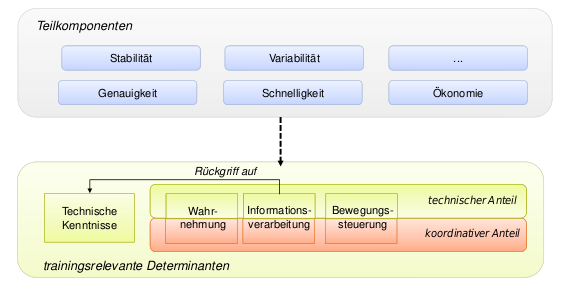
\includegraphics[width=\textwidth]{pictures/tech_determinanten}

\subsubsection*{Phasen des Technikerwerbs}

Das Freiheitsgradproblem:
\begin{itemize}
    \item „Erfunden“ von Nikolai Alexandrowitsch Bernstein, russ. Physiologe, 1896-1966
    \item Problem: Der Mensch hat 880 größere Muskeln!
    \item Wie können diese koordiniert werden?
    \item Motorisches Lernen wird als das Erlernen der Kontrolle von Freiheitsgraden interpretiert: Phasen des motorischen Lernens
\end{itemize}

Phasen des Technikerwerbs:
\begin{enumerate}
    \item Phase ``Freezing'': Einfrieren der Freiheitsgrade
    \begin{itemize}
        \item Freiheitsgrade: Einschränkungen der Muskelgruppen, beteiligter Gelenke, Ausdehnung der Bewegung
        \item Gestalt: geführte Bewegungen, misslingen zunächst öfter
        \item Methodik: Komplexitätsreduktion, Gelegenheit zur Auseinandersetzung geben: Ermüdung, Rückmeldung
    \end{itemize}
    \item Phase ``Releasing'': Befreien der Freiheitsgrade
    \begin{itemize}
        \item Freiheitsgrade:Sukzessives Freisetzen, „selective defrosting“
        \item Gestalt: flüssige, lockere Bewegung, Kombinationen
        \item Methodik: Intensive Rückmeldungen, große Wiederholungszahlen
    \end{itemize}
    \item Phase ``Exploiting'': Ausbeuten der Freiheitsgrade zur Anpassung, Optimierung
    \begin{itemize}
        \item Freiheitsgrade: Ausnutzen, um dynamisches Optimum zu realisieren
        \item Gestalt: oft DVZ, Absprung-, Aushol-, Schlagbewegungen
        \item Methodik: Wann wird zur Ausbeutung gegriffen? Erhöhte Belastung bedenken!
    \end{itemize}
\end{enumerate}

\subsubsection*{Motor Learning}

Lernarten:
\begin{itemize}
    \item Soziales oder Modelllernen: Lernen vom Vorbild, Star, Lehrer, Vormachen-Nachmachen
    \item Versuch-Irrtum-Lernen: Explorierendes Lernen, Implizites Lernen, Bedeutung oft unterschätzt, Anfänger: keine hinreichende Bewegungsvorstellung, Könner: Gegenstand zu differenziert
    \item Lernen durch Einsicht: Zirkel: Instruktion-Durchführung-Ext./Int.Feedback-Bewegungsvorstellung, Umfang und Bedeutung oft überschätzt, Basis des traditionellen methodischen Vorgehens
\end{itemize}

Methodische Übungsreihen (MÜR):
\begin{itemize}
    \item ``Methodische Übungsreihen sind nach methodischen Grundsätzen geordnete Übungsfolgen, die zur Erlernung einer bestimmten motorischen Fertigkeit (Zielübung) ... führen sollen''
    \item Goldstandard des lehrerzentrierten Sportunterrichts
    \item Typen: Aufgliederung in Teilbewegungen, graduelle Annährung, verminderte Lernhilfen
    \item Anordnungsprinzipien: von einfach zu komplex, von leicht zu schwer
\end{itemize}

Neue Ansätze im motorischen Lernen:
\begin{itemize}
    \item bisherige Modelle zu kognitionslastig
    \item Wahrnehmng und Kontext zu wenig berücksichtigt
    \item Bewegungen werden als Antworten auf Umweltkonstellationen interpretiert: ``Constraints'': Einschränkungen der Möglichkeiten, ``Affordances'': Bewegungsmöglichkeiten, diese Wahrnehmung überwiegend unbewusst
    \item Systemdynamischer Ansatz:
    \begin{itemize}
        \item es gibt keine zentrale kortikale Kontrollinstanz zur Bewegungssteuerung
        \item folglich bilden bewusste Prozesse lediglich einen Rahmen für die Bewegungsausführung und sind für die Bewegungskontrolle wenig bedeutsam
        \item Kontrolle wird an dezentrale ``koordinative Strukturen'' delegiert
    \end{itemize}
    \item Ecological approaches: Bewegug wird in einem chaotischen Prozess und in Abhängigkeit von den wechselnden Umweltbedingungen meist unbewusst jedes mal neu generiert. Bewegungslernen = unbewusste Selbstorganisationsprozesse
    \item Implizites Lernen:
    \begin{itemize}
        \item unbewusstes Lernen, ohne Aufmerksamkeit
        \item inzidentell: Unbeabsichtiges Lernen durch Konfrontation mit Lernsituation, Erfolg nicht herbeiführbar (Straßenfußballer-Hypothese)
        \item erfordert intensive und umfangreiche Beschäftigung und hohe Motivation
        \item experimentelle Befunde in der Psychologie
        \item besonders geeignet für komplexe und nicht zu verbalisierende Lerngegenstände
    \end{itemize}
\end{itemize}

Indikationen:
\begin{description}
    \item [Explizit / intentional] bewusstseinspflichtige (erste Lernphasen?) und bewusstseinsfähige Inhalte (Spielzüge, Konzeptionen, Standardsituationen), besonders in kompositorischen und konditionellen Sportarten
    \item [Implizit / inzidentell] komplexe und immer neue Situationen, besonders Sportspiele und Kampfsportarten
\end{description}

\subsection{Trainingsmethoden}

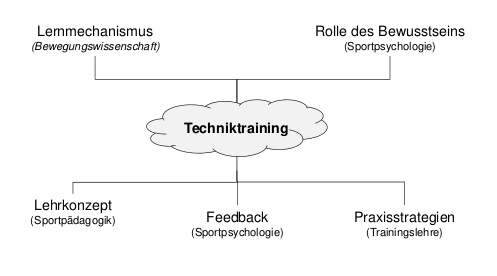
\includegraphics[width=\textwidth]{pictures/tech_mindmap}

\subsubsection*{Lernmechanismus (Bewegungswissenschaft)}

Theorien zum motorischen lernen (die zweite):
\begin{itemize}
    \item Operande Konditionierung (Skinner, 1955): ML ist das Antrainieren von Reflexen auf Umweltreize
    \item Freezing, Releasing, Exploiting (Bernstein,1967): ML ist die Kontrolle von Freiheitsgraden
    \item Motorisch Programme (Schmidt, 1974): ML ist der Aufbau von zentral steuerbaren motorischen Programmen
    \item Theorie der Sensomotorik (Ungerer, 1977): ML ist das Verknüpfen „motorischer Elementarzeichen“ zu Bewegungssequenzen
    \item Ökologische Ansätze (Gibson, 1979, Turvey, 1977): ML ist ein unbewusster Selbstorganisationsvorgang als Antwort auf Umweltwahrnehmungen
\end{itemize}

Lernen durch \ldots:
\begin{itemize}
    \item Konditionierung: Antrainieren von Reflexen (z.B. Deckung beim Boxen), Abtrainieren (Habituation) von Reflexen (z.B. Handballtorwart), Einüben von Bewegungsrhythmen (Stemmschritt)
    \item Imitation: z.B. Fotos, Bildreihen, Videoaufnahmen, Vormachen des Trainers, Beobachtung von anderen Sportlern
    \item Einsicht: Gedankliche Auseinandersetzung mit der eigenen Bewegung, Suchen nach und Erkennen von Fehlern, Erfassen von Ursache und Wirkung, Erarbeitung einer Lösung
    \item Versuch und Irrtum: Lernen muss weitgehend ohne externe Kontrolle/Korrektur funktionieren (z.B. Muttersprache, grundlegende Motorik), Motivation ist nicht das Lernen an sich sondern die Erreichung eines Zieles, Selbständiges Suchen nach Lösungen, Rückschläge in Kauf nehmen, Lernen geschieht hierbei nebenläufig und unbewusst (implizit)
\end{itemize}

\subsubsection*{Lehrkonzept (Sportpädagogik)}

Explizites Techniklernen:
\begin{itemize}
    \item Technik wird wie ein Produkt in mehreren Schritten bewusst (=intentional) ``hergestellt'' (=technologische Position)
    \item Lernen durch Konditionierung, Einsicht, Modellernen, extrinsisches Feedback
    \item Gedankliche Erfassung der Bewegung $\rightarrow$ Beherrschen der Grobform $\rightarrow$ Variation, Stabilisation, Abschirmung
    \item Kritik: ``Kids in America grow up playing in the parks. In Germany they come to the clubs and have practice and stuff like that!''
\end{itemize}

Implizites Techniklernen:
\begin{itemize}
    \item Beiläufiges, ``natürliches'' Lernen ohne Lernabsicht am Einzelfall (=inzidentell)
    \item Antrieb ist eine realen Situation zu lösen
    \item intensive und umfangreiche Beschäftigung, höchst motiviert
    \item Lernen durch Versuch \& Irrtum
    \item ``Freies, unangeleitetes Spielen führt zu Verbesserungen der technischen und taktischen Leistungsvoraussetzungen und ist expliziten Methoden teilweise sogar überlegen'' (Straßenspielerhypothese)
    \item Kritik: Straßenspiel ist zu wenig steuerbar, zu langsam, Erfolg ist unsicher
\end{itemize}

\subsubsection*{Rolle des Bewusstseins (Sportpsychologie)}



\subsubsection*{Feedback (Sportpsychologie)}

\subsubsection*{Praxisstrategien (Trainingslehre)}

\subsection{Trainingsinhalte}

\subsection{Anwendung}

\subsection{Diagnostik}



\newpage
%!TEX root = ../report.tex
\section{Taktik}

\subsection{Begriffe \& Systematik}
\begin{description}
  \item[Taktik] ist ein System von Handlungsplänen und Entscheidungsalternativen, das Trainings- und Wettkampfverhalten so zu regulieren gestattet, dass ein optimaler sportlicher Erfolg möglich wird.
  \item[Strategie] ist über längere Zeit gesehene Taktik.
  \item[Taktisches Verhalten] bedeutet eine Situation mit einer Handlung zu beantworten
  \item[Taktisch entscheiden] bedeutet in einer Situation aus einer Menge aus Alternativen einen Handlungsplan auswählen. Es existieren verschiedene Kopplungsmodelle dieses Auswahlverfahrens: Feste Assoziation (eine Situation impliziert genau eine Handlung), Auswahl aus Alternativen (eine Situation kann eine Gruppe von Handlungen implizieren), Vorsatzhandlungen (es existiert nur eine Handlungsalternative).
\end{description}
\begin{figure}[H]
  \begin{flushleft}
    \textbf{Systematisierung nach Zeit}
  \end{flushleft}
  \centering
  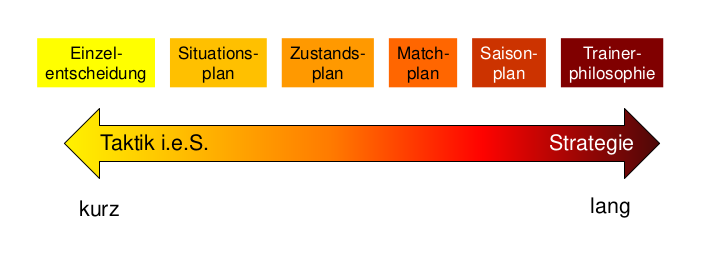
\includegraphics[width=.7\textwidth]{pictures/taktik_systematisierung.png}
  \caption{Systematisierung von Taktik nach Zeit}
\end{figure}
\paragraph{Systematisierung nach \# beteiligter Spieler} Taktik kann abhängig von der Anzahl der Spieler eingeteilt werden. Teilbereiche sind dann Mannschaftstaktik, Gruppentaktik und Individualtaktik.
\paragraph{Systematisierung nach Spielsituation} Mögliche Varianten sind Standardsituation, Offensivtaktik, Defensivtaktik, Übergangsphasen
\paragraph{Systematisierung nach Trainingszielen}
\begin{itemize}
  \item Taktische Kenntnisse: Wissensbestände, deklaratives Wissen
  \item Taktische Fähigkeiten: Situationsübergreifende taktische Handlungskompetenz: Wahrnehmung, Entscheidung, Ausführung
  \item Taktische Fertigkeiten: Angemessene und erfolgreiche Antworthandlungen (Individuell, teilkollektiv und kollektiv)
\end{itemize}
\paragraph{Taktische Handlungsphasen (nach Heckhausen)}
\begin{enumerate}
  \item Prädezisionale Phase: Wählen/ Entscheiden
  \item Präaktionale Phase: Planen/ Abschirmen
  \item Aktionale Phase: Ausführen
  \item Postaktionale Phase: Vergleichen/ Bewerten
\end{enumerate}
\begin{figure}[H]
  \begin{flushleft}
    \textbf{Phasenstruktur taktischen Handelns (nach Mahlo)}
  \end{flushleft}
  \centering
  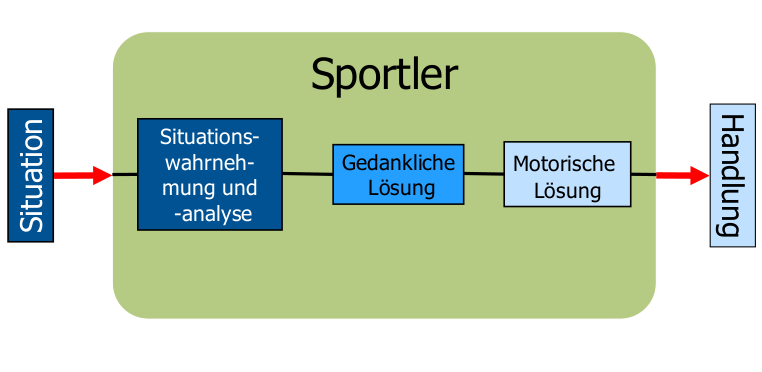
\includegraphics[width=.7\textwidth]{pictures/taktik_phasenstruktur_des_handelns.png}
\end{figure}
Probleme dieses Ansatzes:
\begin{itemize}
  \item Werden die Phasen vollständig durchlaufen?
  \item Werden die Phasen nacheinander druchlaufen?
  \item Entscheidungen werden bewusst getroffen
\end{itemize}
\paragraph{Fehlerquellen bei taktischen Entscheidungen} Taktische Fehlentscheidungen können durch alle 3 Phasen enstehen. Falsche Situationswahrnehmung und -analyse (sensorische Probleme), Inkorrekte gedankliche Lösungen (Wahl der falschen Alternative, Menge an Vorerfahrung, akt. Einflüsse) und eine mangelnde motorische Umsetzung (Fehleinschätzung der Fähigkeiten, situative Umstände)
\paragraph{Entscheidungsmodelle der Psychologie}
\begin{itemize}
  \item Zufallsentscheidung
  \item Heuristische Entscheidung
  \item Rational-Choice Entscheidung: viele Theorien, z.B.\ Erwartungs-mal-Wert-Therie (Probleme: alle Alternativen, Werte \& Wahrscheinlichkeiten bekannt?)
\end{itemize}
\paragraph{Aktuelle Theorien - Top-down \& Bottom-up Prozesse}
\begin{description}
  \item[Top-down Prozesse] Kognitionsgesteuerte, verbalisierbare Erwartungs- und Zielbildungsprozesse (Wenn A dann B)
  \item[Bottom-up Prozesse] Wahrnehmungs- gesteuerte, nicht verbalisierbare Wahrnehmungs- Handlungsprozesse. (Reaktionen)
\end{description}
Mögliche Zusammenspiele der beiden Prozesse:\\
\begin{minipage}{0.1\textwidth}
  
\includegraphics[width=\textwidth]{pictures/taktik_top-down_bottom-up.png}
\end{minipage}
\begin{minipage}{0.9\textwidth}
  \begin{itemize}
    \item Selektion: Nur je ein Typ aktiv (Vorsatzhandlungen)
    \item Konkurrenz: 1 Typ dominiert, i.d.R.\ Top-down (einfache Situationen)
    \item Kooperation: beide in gleiche Richtung (komplexe Situationen)
    \item Korrektur: Wahrnehmung korrigiert Entscheidung
  \end{itemize}
\end{minipage}
Top-down Prozesse sind explizit lehrbar, Bottom-up nicht/nur implizit. Lehren von Top-down Prozessen beinhaltet taktisches Wissen, Spielsysteme, Standardsituationen und Vorsatzhandlungen. Implizites Botto-up Training beinhaltet das Verhalten im Raum, das Erkennen von Optionen, Lesen des Gegners und die Lösung von Situationen.

\subsection{Determinanten}
\begin{figure}[H]
  \centering
  \begin{subfigure}{.45\textwidth}
    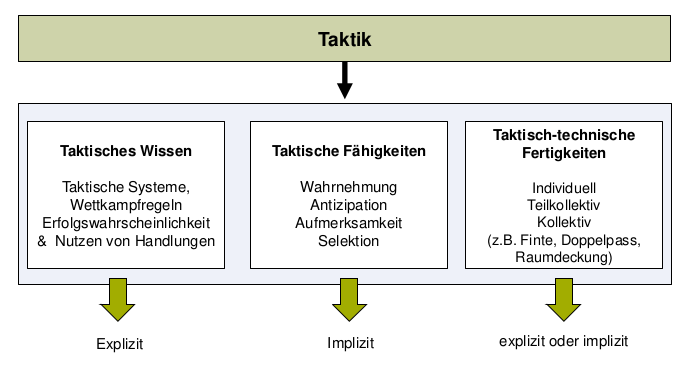
\includegraphics[width=\textwidth]{pictures/taktik_determinanten.png}
    \caption{Allgemeine Determinanten}
  \end{subfigure}
  \begin{subfigure}{.45\textwidth}
    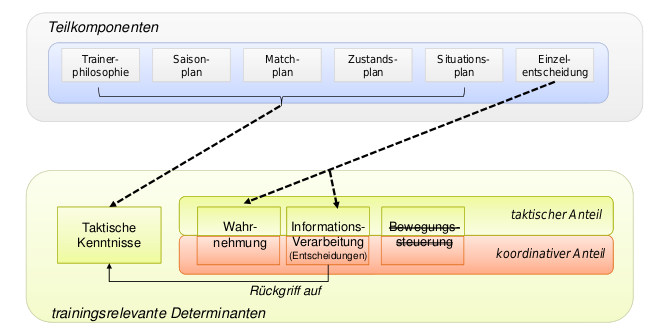
\includegraphics[width=\textwidth]{pictures/taktik_determinanten_trainingsrelevant.png}
    \caption{Trainingsrelevante Determinanten}
  \end{subfigure}
\end{figure}

\subsection{Trainingsinhalte}
Taktische Kenntnisse $\rightarrow$ Wissensvermittlung\\
Realisation von geplanten Spielzügen $\rightarrow$ Abstimmung zwischen Mannschafften\\
Situatives Lösen von offenen Situationen $\rightarrow$ Korrektheit und Schnelligkeit der taktischen Entscheidung
\paragraph{Rolle des Bewusstseins} Bewusstseinspflichtige Inhalte (z.B.\ Regeln) und bewusstseinsfähige Inhalte (z.B.\ Erfolgswahrscheinlichkeit von Handlungen) bilden die taktischen Kenntisse. Zusätzlich gibt es noch nicht-bewusstseinsfähige Inhalte (z.B.\ schnelle Entscheidungen) die nicht zur Taktik zählen.
\paragraph{Vermittlungskonzepte}
\begin{itemize}
  \item Explizit/Intentional: Systematisches Lernen\\
    Beispielhafte Übungsreihe:\\
    \begin{tabular}{m{0.4\textwidth} | m{0.4\textwidth}}
      Stufen & Inhalt \\ \hline
      Isoliertes Üben der Handlungsalternative A & Üben mit fest vorgegebenem Verhalten A \\ \hline
      Isoliertes Üben der Handlungsalternative B & Üben mit fest vorgegebenem Verhalten B \\ \hline
      Entscheidungstraining\newline Handlungsalternative A oder B? & Üben, bei dem überwiegend Abwehrverhalten A \newline gezeigt wird und nur selten Abwehrverhalten B \\ \hline
      Handlungsalternative B oder A? & Üben, bei dem überwiegend Abwehrverhalten B\newline
      gezeigt wird und nur selten Abwehrverhalten A \\ \hline
      Isoliertes Übender Handlungsalternative C & Üben mit fest vorgegebenem Verhalten C \\ \hline
      Entscheidungstraining & \ldots \\ \hline
      Wettkampfnahes Spieltraining/Anwendung im Wettspiel & Üben mit nicht eingeschränkten Gegnerverhalten \\
    \end{tabular}
  \item Implizit/Inzidentell: Unbewusstes Lernen am Einzellfall (mit Vorgabe der Rahmenbedingungen.\\
    Menschen lernen Dinge unbewusst ohne explizite Erklärung. Dafür wird vor Allem intrinsische Motivation genötigt, ansonsten kein Fortschritt.
\end{itemize}
\textbf{Theorie der antizipativen Verhaltenskontrolle nach Hoffmann}\newline
  \begin{minipage}{.5\textwidth}
  In einer Ausgangsbedingung ($S_{Augs}$) werden Konsequenzen ($K_{Ant}$) des eignen Handelns (R) antizipiert und mit real eingetroffener Konsequenz ($K_{Real}$) verglichen.
  Bei Gleichheit wird die Assoziation verstärkt, ansonsten findet eine Neubewertung der Ausgangssituation statt.\\
  Lernen besteht darin, die Differenzen durch Restrukturierung der Äquivalezklassen zu minimieren.
  Die AVK (d.h.\ die Einteilung in die einzelnen Teilabschnitte) ist anwendbar für den ganzen Bereich von Bottom-up zu Top-down Prozessen.
  \end{minipage}
  \begin{minipage}{.5\textwidth}
    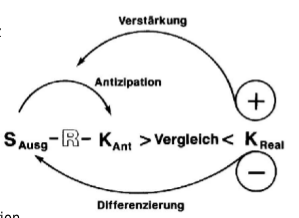
\includegraphics[width=\textwidth]{pictures/taktik_avk.png}
  \end{minipage}

\subsection{Trainingsmethoden}
\paragraph{Grundsätze}
\begin{itemize}
  \item Ähnliche, homogene Situationen schaffen und Assoziationen mehrfach bestätigen
  \item Verhaltensziele nicht IMMER erreichen, zur Differenzierung von Situationen
  \item Komplexitätssteigerung für Grenzfälle
  \item Explizite Hinweise, z.B.\ Anzeigen von Handlungsmöglichkeiten
  \item Realistische Entscheidungsalternativen
\end{itemize}
\begin{figure}[H]
  \begin{flushleft}
    \textbf{Abgrenzung Schelligkeits-, Koordinations- \& Taktiktraining}\\
  \end{flushleft}
  \centering
  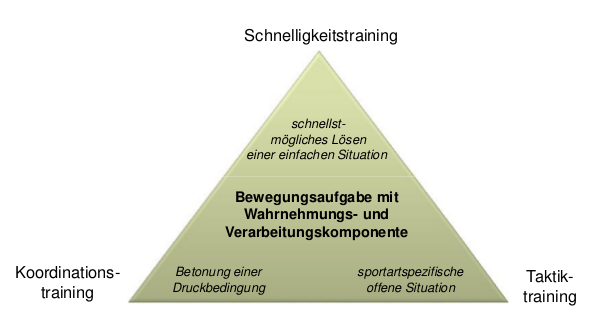
\includegraphics[width=.7\textwidth]{pictures/taktik_training_abgrenzung.png}
\end{figure}

\subsection{Anwendung}
\begin{tabular}{p{.3\textwidth} | p{.3\textwidth} | p{.3\textwidth}}
  & Pro & Contra \\ \hline 
  Explizit & 
    \begin{itemize}[noitemsep,nolistsep]
      \item gezielt, systematisch
      \item kann sofort wirken
    \end{itemize} &
    \begin{itemize}[noitemsep,nolistsep]
      \item Explosion von Regeln
      \item Verlust von Detailinformationen
      \item gebunden an Aufmerksamkeit, vergessensanfällig
      \item behindert Einsicht, Kreativität
    \end{itemize}\\ \hline
  Implizit & 
    \begin{itemize}[noitemsep,nolistsep]
      \item Praxisevidenz
      \item Intrinsische Motivation
    \end{itemize} & 
    \begin{itemize}[noitemsep,nolistsep]
      \item Erfolg nicht unmittelbar herbeiführbar.
      \item langsam
      \item schlechte Belegbarkeit
    \end{itemize}\\ \hline
\end{tabular}

\subsection{Diagnostik}
\paragraph{Spielanalyze} ist eine analytische, zielgerichtet Beschreibung und Interpretation des Verhaltens im Sportspiel zum Zweck der Leistungsdiagnose.
Es gibt 2 methodische Grundtypen:
\begin{description}
  \item[Quantitativ] Verhalten wird auf ein Beobachtungssystem abgebildet, die Ergebnisse sind konkrete Zahlen.
    \begin{itemize}
      \item Beobachtungssystem: Struktur der zu erhebenden Daten in einem Modell
      \item Beobachtungseinheit: Elementarereignis (z.B.\ Ballkontakte)
      \item Beobachtungsmerkmal: Eigenschaft einer Beobachtungseinheit (z.B.\ Spieler, Annahmequalität)
      \item Merkmalsausprägungen: Arten, wie ein Merkmal auftreten kann (z.B.\ gut, schlecht, 42cm)
      \item Typen von Ausprägungen (z.B.\ Nominalmerkmale, Ganzzahl)
    \end{itemize}
  \item[Qualitativ] Geschehen wird beobachtet mit eigener Expertise verglichen, die Ergebnisse sind Einschätzungen und Interpretationen.
\end{description}

\subsection{Zusammenfassung}

\newpage
%!TEX root] ../report.tex

\section{Trainingsmodelle}

Generell:
\begin{description}
    \item[kurzfristig] Leistungsveränderungen durch optimale Gestaltung der Einzelreize anstoßen
    \item [mittelfristig] Leistungsfähigkeit steigern und herausbilden der optimalen Form für einen bestimmten Zeitraum
    \item [langfristig] Leistungspotential langfristig ausschöpfen
\end{description}

\subsection{kurzfristig}

Grundlegende Begriffe:
\begin{description}
    \item [Homöostase] dauerhaft aufrechthaltbarer Gleichgewichtszustand in Ruhe
    \item [Heterostase] Störung der Homöostase
    \item [Belastung] objektiv von Außen auf den Organismus wirkende Faktoren Umstellung] Zustandsveränderung der Funktionssysteme im Rahmen ihres Regulationsbereiches durch Belastung (auch Aktivierung)
    \item [Beanspruchung] individuelle Reaktion des Organismus auf eine Belastung
    \item [(Max) Steady State] zeitlich begrenzt aufrechthaltbare (maximale) Leistung während der Belastung
    \item [Ermüdung] reversible Leistungsminderung durch Beanspruchung
    \item [Regeneration] Prozesse zur Wiederherstellung der Homöostase
    \item [Superkompensation] überschießende Wiederherstellung der Leistungsfähigkeit
    \item [Adaptation] zeitlich stabile, reversible Steigerung der Leistungsfähigkeit durch Beanspruchung
    \item [Deadaptation] Rückbildung der Leistungsfähigkeit durch fehlende Beanspruchung
\end{description}

\newpage
%!TEX root = ../report.tex
\section{Trainingssteuerung}
Trainingssteuerung ist die gewichtete kurz-, mittel- und langfristige Abstimmung und Ausführung aller Planungs-, Trainings-, Kontroll-, Auswertungs- und Lenkungsmaßnahmen eines Trainingsprozesses zur Erreichung der Trainingsziele.
\begin{figure}[H]
  \centering
  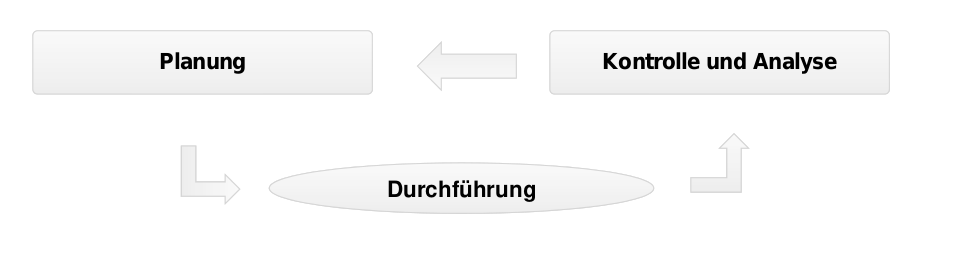
\includegraphics[width=.7\textwidth]{pictures/trainingssteuerung_komponenten.png}
\end{figure}

\subsection{Planung}
\begin{figure}[H]
  \centering
  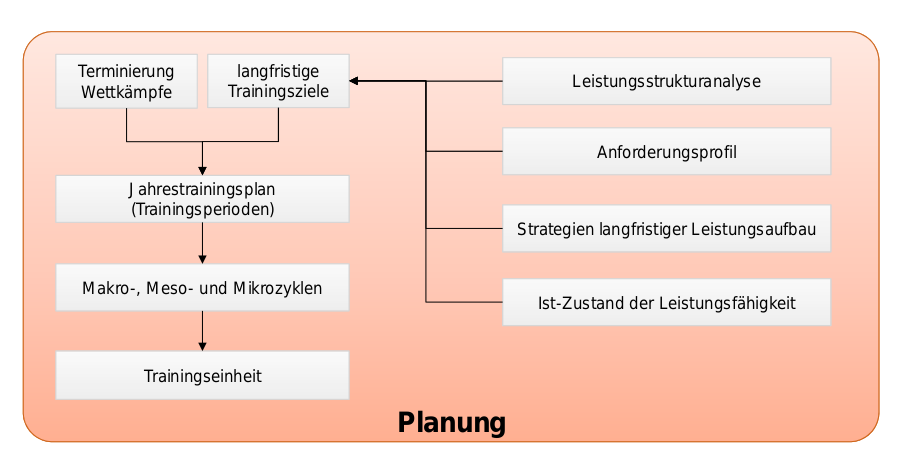
\includegraphics[width=.7\textwidth]{pictures/trainingsplanung_komponenten.png}
\end{figure}
\paragraph{Leistungsstrukturanalyse} Analyse aus welchen Komponenten die Leistung einer Sportart besteht.
Davon werden diejenigen ausgewählt, die besonders entscheidend für den Erfolg sind und werden maximiert.
Die übrigen nur optimiert.\\
\paragraph{Anforderungsprofil} beschreibt wie gut Fähigkeiten auf dem angestrebten Niveau ausgeprägt sein müssen.
Beinhaltet sind:
\begin{itemize}
  \item Leistungsnorm: ist die resultierende Wettkampfleistungen/Teilleistungen
  \item Konditionelle Norm
  \item technisch-taktische Norm
\end{itemize}
\paragraph{Langfristige Traingingsziele} werden mithilfe der Leistungsstrukturanalyse, dem Anforderungsprofil, der Wettkampfanalyse \& der Trainerphilosophie gesetzt.
Folgende fragen sind wichtig:
\begin{itemize}
  \item Ist die Trainierbarkeit gegeben? (Reaktionsschnelligkeit, Kraft)
  \item Lohnt sich das Training? (Abwägung von Niveau, Potential und Zeitbuget)
  \item Ist eine Integration in das Training möglich? (Konkurrenz der verschiedenen Komponenten im Zeitbuget, Wechselwirkungen der Komponenten)
\end{itemize}
\textbf{Planung einer Trainingseinheit}\\
\begin{figure}[H]
  \centering
  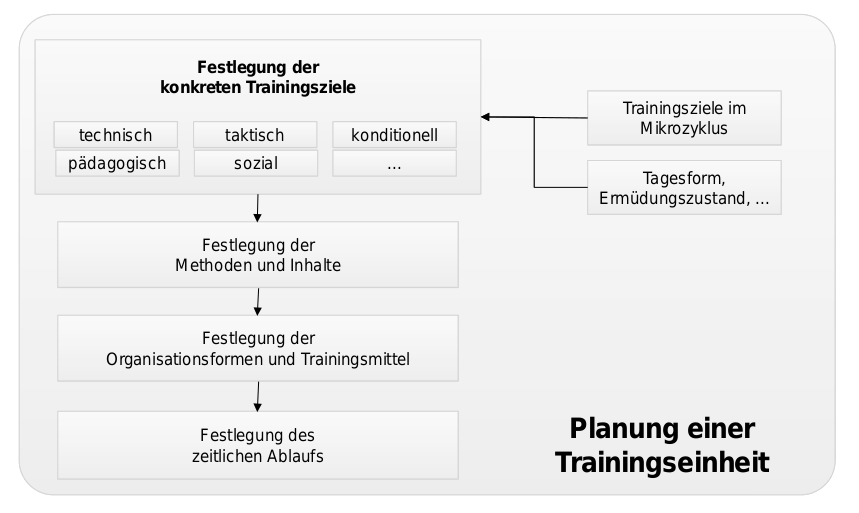
\includegraphics[width=.7\textwidth]{pictures/trainingssteuerung_planung_trainingseinheit.png}
\end{figure}
\begin{figure}[H]
  \centering
  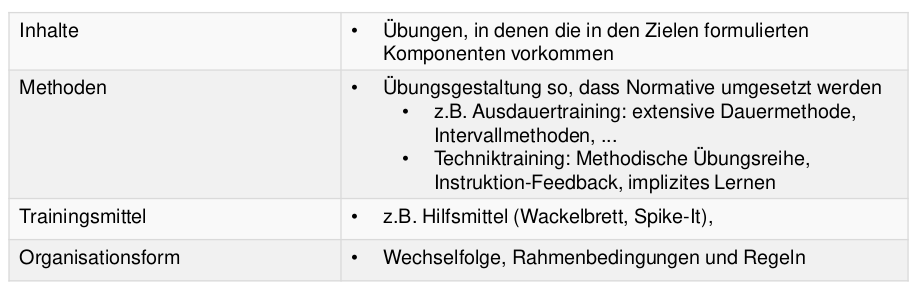
\includegraphics[width=.7\textwidth]{pictures/trainingssteuerung_planung_trainingseinheiten_komponenten.png}
\end{figure}
Zieldefinition:\\
\begin{figure}[H]
  \centering
  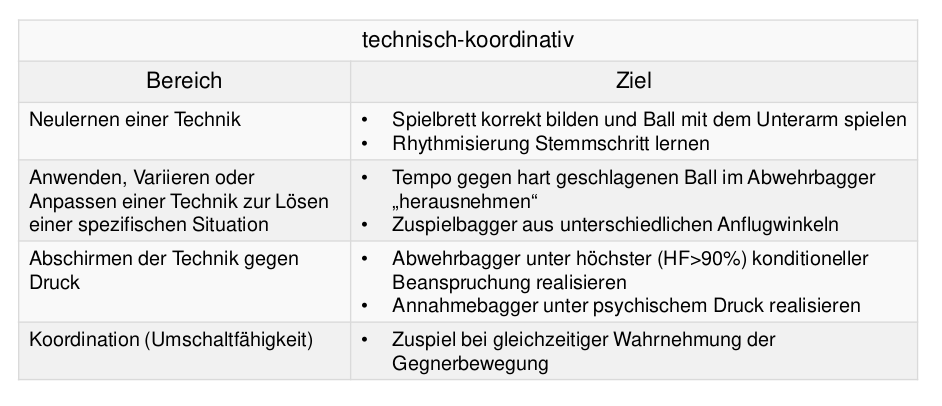
\includegraphics[width=.7\textwidth]{pictures/trainingssteuerung_zieldefinition_koordinativ.png}
\end{figure}
\begin{figure}[H]
  \centering
  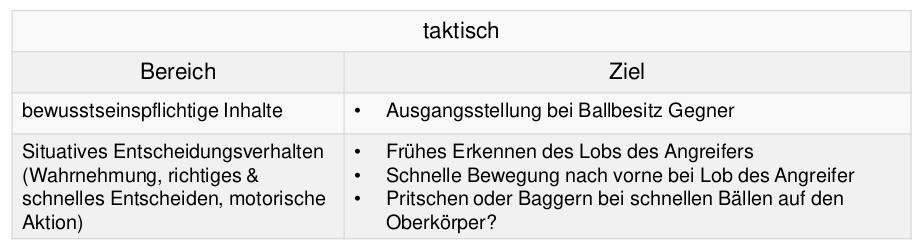
\includegraphics[width=.7\textwidth]{pictures/trainingssteuerung_zieldefinition_taktisch.png}
\end{figure}
\begin{figure}[H]
  \centering
  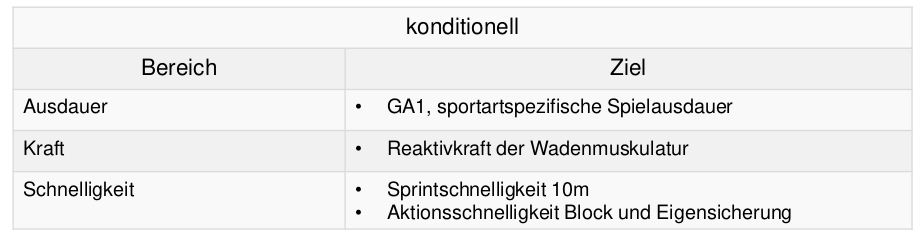
\includegraphics[width=.7\textwidth]{pictures/trainingssteuerung_zieldefinition_konditionell.png}
\end{figure}
Zeitlicher Ablauf einer Trainingseinheit:\\
Der Ablauf ist üblicherweise in drei Teile eingeteilt: Ein einleitender Teil, in dem eine mentale und physische Vorbereitung erfolgt, ein Hauptteil, in dem die Trainingsziele umgesetzt werden sollen und den Ausklang, in dem die Regeneration eingeleitet wird.\\
Im Hauptteil werden zunächst die Trainingsziele umgesetzt, die eher einen erholten Zustand erfordern, wie Schnelligkeit, Koordination oder Reaktion.
Gegen ende des Trainings werden dann vermehrt die anstrengenderen Trainingsziele in betracht gezogen, wie aerobe Ausdauer, Kraftausdauer oder Techniktrainingsabschrimung.

\subsection{Durchführung}
Kritisch überprüfen, ob Training wie geplant abläuft!
\begin{itemize}
  \item Technisch-Taktisch
    \begin{itemize}
      \item Entstehen die benötigten Situationen ausreichend häufig?
      \item Können Techniken in der Situation sinnvoll angewendet werden?
      \item Sind Entscheidungen richtig?
      \item Ist Feedback vorhanden?
    \end{itemize}
  \item Konditionell
    \begin{itemize}
      \item Werden die Normative erreicht (Belastung zu hoch, zu niedrig)? evtl.
      \item Pulskontrolle
      \item Sind Pausen zu lang, zu kurz?
      \item Intensitätssteuerung schwierig -> "mündiger Athlet" (Lenk)
    \end{itemize}
  \item Durchführung ggf.\ verändern (z.B.\ Organisationsform)
\end{itemize}

\subsection{Kontrolle und Analyse}
Es gibt drei verschiedene Arten von Diagnositken:
\begin{itemize}
  \item Leistungsdiagnostik ist die Beschreibung und Beurteilung der Leistung, der Teilleistungen und Leistungskomponenten. Erfasst werden Wettkampf(teil-)leistungen oft über spezielle motorische Tests.
  \item Wettkampfdiagnostik ist Leistungsdiagnostik im Wettkampf oder unter Wettkampfbedingungen
  \item Trainingsdiagnostik ist die Beschreibung und Beurteilung des Trainingsprozesses und seiner Wirkung (nicht Leistungsdiagnostik im Training).
    Dabei werden Trainingskomponenten wie Belastungen und Beanspruchungen erfasst.
    Komponenten:\\
    \begin{figure}[H]
      \centering
      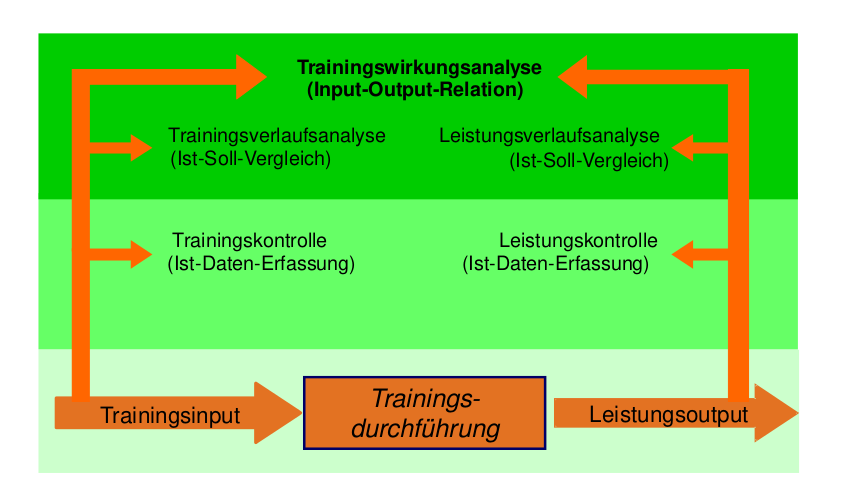
\includegraphics[width=.7\textwidth]{pictures/trainingssteuerung_trainingsdiagnostik_komponenten.png}
    \end{figure}
\end{itemize}

\newpage
%!TEX root = ../report.tex
\section{Leistungsdiagnostik}
Leistungsdiagnostik ist die Feststellung der Wettkampfleistung, von Wettkampf-Teilleistungen und von Leistungsvoraussetzungen.
Die Messung der Leistungsvorraussetzungen erfolgt über motorische Tests, leistungsphysiologische Verfahren (Laktat), biomechanische Verfahren (Laufanalysen) und psychologische Verfahren.
Die Messung der Wettkampfleistung über biomechanische Messungen (von einzelnen Läufen), Wettkampfdokumentationen und Spielbeobachtungen.

\subsection{Theoretische vs.\ Praktische Leistungsdiagnostik}
\paragraph{Theoretische Leistungsdiagnostik (TLD)}
Leistungsdiagnostik zum Zweck der Erstellung allgemeiner Aussagen über die Leistungsstruktur einer Sportart.\\
Typische TLD Fragestellungen:
\begin{itemize}
  \item Allgemeine Modellierung der sportlichen Leistung
  \item Sportartspezifische Modellbildung
  \item Alters- und Geschlechtsabhängigkeit der Leistungsstruktur
  \item Abhängigkeit der Leistungsstruktur vom Leistungsniveau
  \item Erstellung statistischer Normen
\end{itemize}
\paragraph{Praktische Leistungsdiagnostik (PLD)}
Leistungsdiagnostik im Kontext eines Trainingsprozesses.
PLD diagnostiziert die Wettkampfleistung und den Leistungszustand von Mannschaften und Athleten.
PLD ergängzt die Methoden von TLD mit qualitativen Analyzen von Einzelfällen.
Die Unterschiede von TLD und PLD liegen vorallem darin, dass sich PLD eher mit Einzelfällen und TLD eher für allgemeine, statistische Aussagen interessiert.
Die beiden Methoden beeinflussen sich allerdings: TLD generiert Hintergrundwissen für PLD und PLD liefert die VOrgaben für TLD (Hypothesen, Inspiration für Modelle).


% Needs to be enabled when there are any references.
% \clearpage
% \addcontentsline{toc}{section}{\refname}
% \printbibliography

\end{document}
